\chapter{POTENTIAL DEVELOPMENT SOFTWARE}
\label{ch:software}
\lstset{
	language=python,
	% basicstyle=\small\sffamily,
	numbers=left,
	numberstyle=\tiny,
	% frame=tb,
	columns=fullflexible,
	showstringspaces=false
}
\section{Introduction}

The simultion of systems involving hundreds of atoms using quantum-mechanical calculations are commonplace, due to the success of density functional theory\cite{hohenberg1964_dft,kohn1965_dft} and the availability of many software packages for the calculations such as VASP\cite{kresse1993_vasp,kresse1996_vasp1,kresse1996_vasp2}, ABINIT\cite{gonze2002_abinit,gonze2005_abinit,gonze2009_abinit,gonze2016_abinit}, and Quantum Espresso\cite{giannozzi2009_quantumespresso}.
These electronic-structure calculations have high fidelity, accuracy improving as the description of the exchange correlation energy functional has improved from local density approximation(LDA) to PBE to hybrid methods.
These electronic-structure models allow for simulations of hundreds of atoms which when combined with workflow management software, such as \emph{AFLOW}\cite{curtarolo2012_aflow} and \emph{pymatgen}\cite{ong2013_pymatgen} has given rise to high-throughput computational efforts, which leverage these energy calculators.

As an alternate to electronic structure methods, empirical potentials describe the effects of the valence electron interactions without explicitly describing the electrons themselves.  The simplied descriptions of interatomic interations allow for larger system sizes and longer simulations timeframes than can be accomplished with \emph{ab initio} techniques.  However, these approaches are accompanied by a loss of accuracy compared to electronic structure methods.

In this chapter, a software toolkit for the reproducible, algorithmic development of interatomic potentials for atomic-level simulations using autonomous machine-learning techniques is described.
The Python Potential Optimization Software Package (\emph{pypospack}) is open-access software for the automation of potential development workflows, which leverages the richness of machine learning codes of the python language with ubiquitous molecular dynamics software code, LAMMPS\cite{plimpton1995_lammps}, and the lattice dynamics code, GULP\cite{gale2003_gulp}.

\subsection{Current state of Potential Development Software}

Classical atomistic simulation methods, of which molecular dynamics (MD) simulation\cite{allen1987_md,haile1992_md,lesar2013_md,frenkel2002_md} is the most common, are a vital tool in the analysis of solid state and materials systems.
The description of the interactions of the atoms is encoded in the interatomic potential, many of which have been developed to describe specific materials systems.
The embedded atom method (EAM)\cite{daw1983_eam,daw1984_eam,daw1993_eam_review,foiles2012_eam_review} and Finnis and Sinclair\cite{finnis1984_fs} potentials, among others, were developed and continue to be developed for metals.
Bond order potentials (BOP) such as those of Brenner\cite{brenner1989_bop,brenner2002_rebo} and Tersoff\cite{tersoff1988_tersoff}, and the three-body Stillinger and Weber\cite{stillinger1985_sw} potential are widely used to describe covalently-bonded materials.
For ionically bonded materials, the electrostatic interactions are typically described by Coulomb potentials, with various formalisms for the short ranged interactions, the Buckingham potential being the most widely used.\cite{lewis1985_buck,gale1996_buck}
The continuing evolution of these formalisms, the development of more sophisticated potential formulations such as ReaxFF\cite{vanduin2001_reaxff,senftle2016_reaxff} and COMB \cite{liang2013_comb_1,liang2013_comb_2}, and the increasing accuracy of density functional theory (DFT) calculations, which typically constitute at least part of the fitting database, have allowed the materials fidelity of these potentials to increase markedly.

\begin{figure}[ht]
	\label{fig:potdev_monolithic}
	\centering
	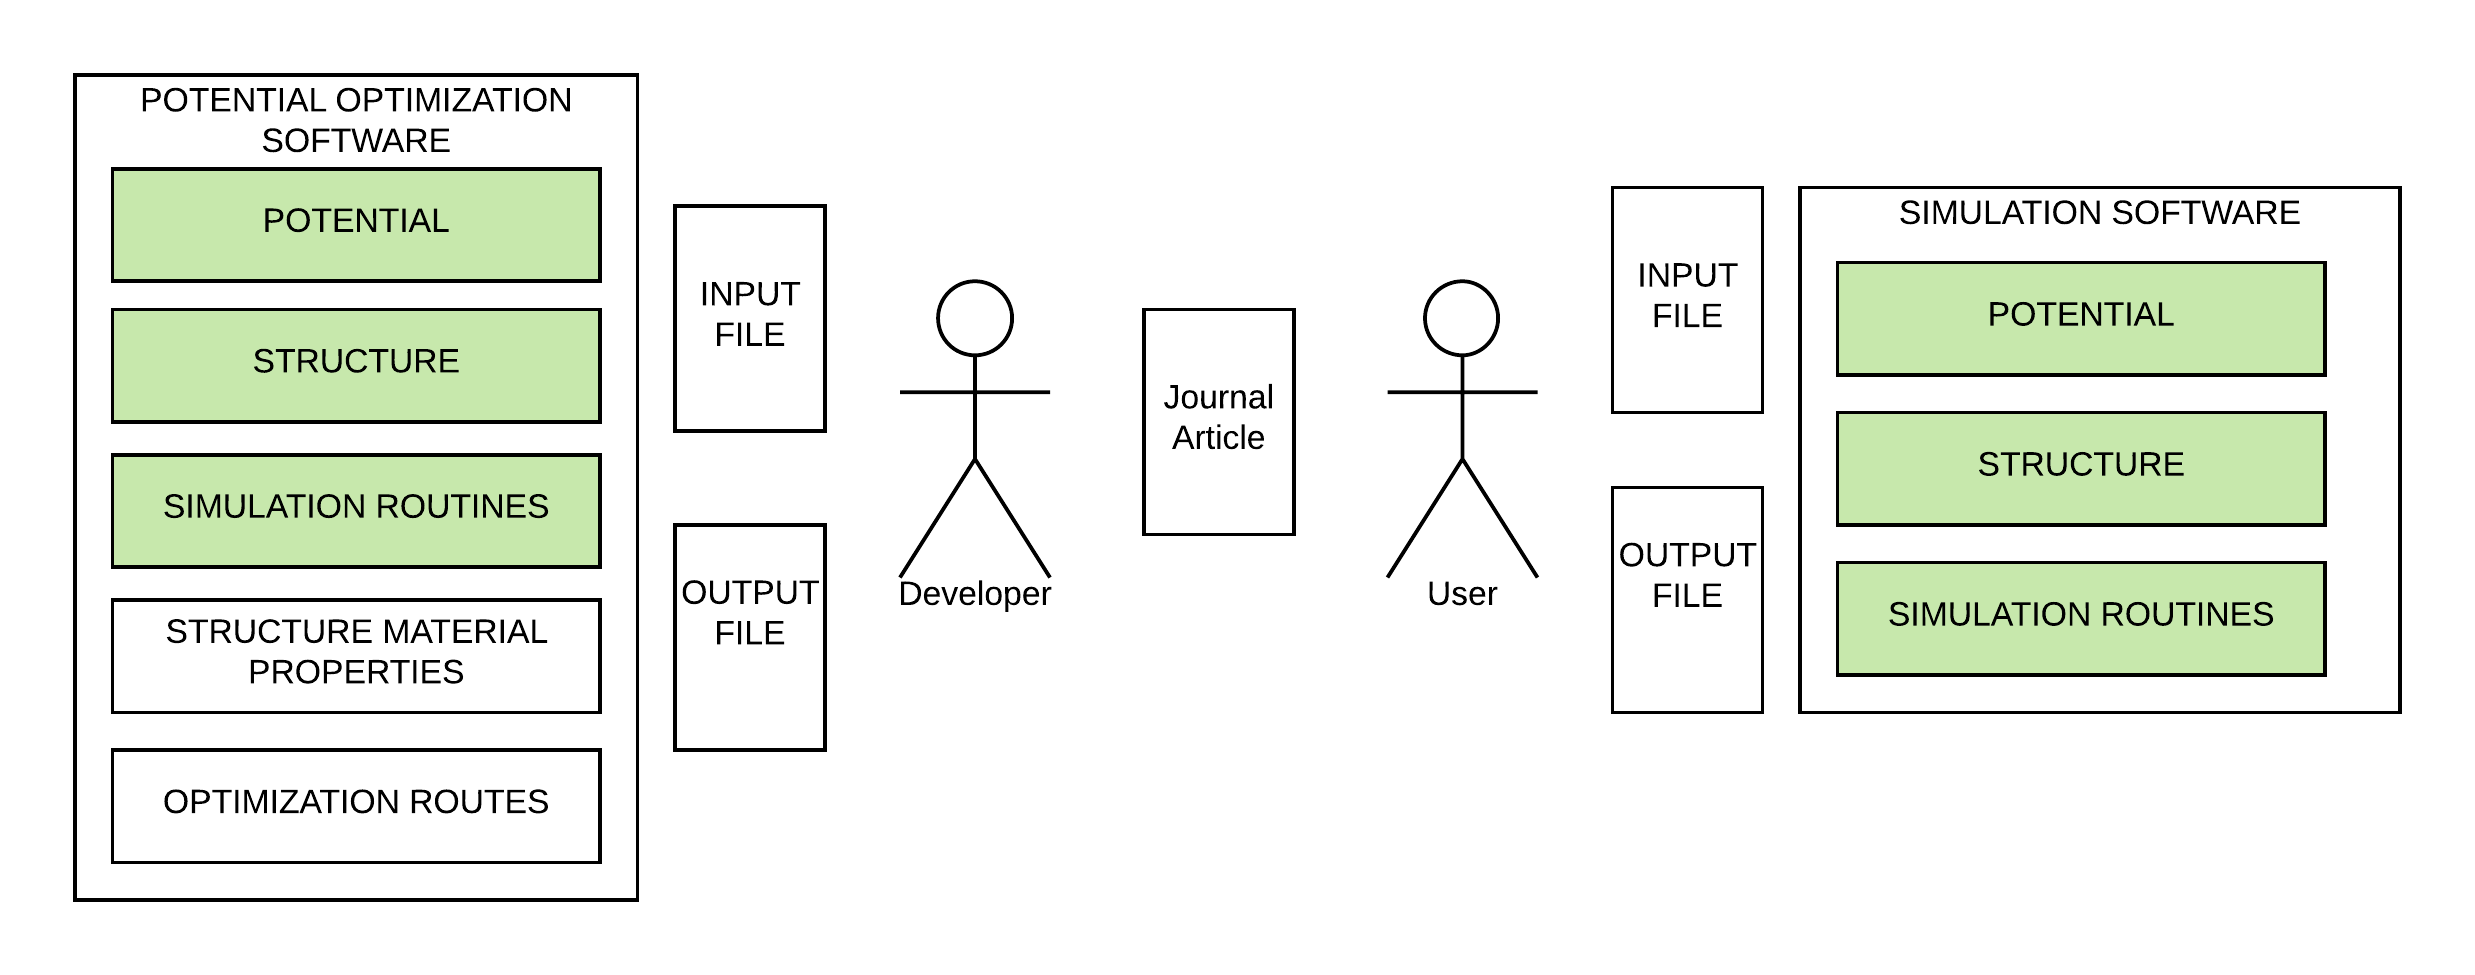
\includegraphics[width=5in]{chapter6/img/fig_potdev_monolithic}
	\caption{Schematic of monolithic potential development software}
\end{figure}

Figure \ref{fig:potdev_monolithic} is a schematic between potential development software, simulation software, the potential developer, and the potential user.  In this software architecture, the code for implementing the potential, the structures, and simulation routines exist both in molecular dynamics software and potential development.

Computational atomistic simulation involves software which have been developed in a variety of different languages, including but not exclusive to C/C++ and Fortran.  The combination of compiler optimization from strict variable typing, well-vetted numerical libraries, and availability of parallelization libraries makes these langagues well-entrenched for the forseeable future.  The most popular atomistic simulation codes have matured over long-periods of time, with significant code contributions from the developers of potential formalisms enhancing the capabilities of the software.

Similarly, potential development software developed iteratively, but with drastically different results.  Early potentials were developed using proprietary simulation codes which were augmented to describe the ability to describe the specific set of simulations to conduct required to optimize a specific set of simulations to calculate structure-property relationships.   In addition, numerical optimization routines to minimize a cost function are described in chapter \ref{ch:potential_development} were necessary to add to the software.  Software codes included the ability to assign weights to the function to encode preferences and evolved to include global optimization techniques, such as simulated annealing\cite{kirkpatrick1983_simmulated_annealing} to deal with the local minima.

Despite the drastic expansion in the amount of formalisms and maturation of simulation codes, potential development software remains tailored to specific potentials and applications.
% Potential software was written which support a small subset of potential formalisms.
Currently, potential software typically supports the development of a small subset of potential formalisms
For example, \emph{POSmat}\cite{martinez2016_posmat} supports the development of COMB potential and \emph{potfit}\cite{brommer2015_potfit} supports the development of embedded atom potentials (EAM).  On the other hand, GULP supports development of potentials based on a relatively small set of material properties.

The monolithic software development model is ill-suited for the demands of potential development.  As indicated in Figure \ref{fig:potdev_monolithic}, the regions in green represents a replication in development effort with simulation codes.  The implementation, maintenance, and update of molecular dynamics code is non-trivial.  However, widely adopted software codes such as LAMMPS have superior support, high reliability, and vetted by ubiquitous use.  More importantly,  there is little incentive for a third-parties to implement new potential formalism to monolithic software development codes.

Discussed in depth in chapter \ref{ch:potential_development}, the final parameterization on depends choices made by the potential developer; this means that the process by which a potential is developed is generally neither fully documented, nor reproducible.  Moreover, there is currently no objective method for evaluating the suitability of the function form of the atomic potential or determining if the final parameterization selected yields the best possible fit to the fitting database.  Current parameterization processes generally involve the minimization of a single scalar cost function, typically the weighted sum of some measure of the difference bewteen the predicted value $\hat{q}_i(\bm{\theta})$ and the reference values of the specific material property $\hat{q}_i$.

As a result, the final parameterization depends on the many choices made by the potential developer; this means that the process by which a potential is developed is generally neither fully documented, nor reproducible.  Nevertheless, the process of potential development largely remains non-transparent and subjective\cite{martinez2013_fitting,martinez2016_posmat}, involving the repeated intervention of a skilled potential developer\cite{brenner2000_fitting}.
This leadsto problems with reproducibility in potential development as the selection of weights and initial conditions are largely not documented in the literature.
As a result, this knowledge is largely proprietary, remains concentrated in potential development groups, and software for potential development remain rudimentary tools developed by the specific needs of potential development groups.

In addition, parameter optimization is dependent upon numerical optimization techniques indicated in orange in Figure \ref{fig:potdev_monolithic}.  As described by Ghosh and Chakraborty \cite{ghosh2014_potdev_pareto}, the general problem of parameter optimization is an application of black box function optimization.  Cost function optimization techniques are unable to obtain compromise solutions which are Pareto efficient if they are occluded within a convex region of performance space.

\subsection{Goals of this Software}

Potential software development is by necessity a complicated, drawing expertise from many disciplines including materials science, numerical analysis, and software development.

The goal of \emph{pypospack} is to provide a flexible software architectural library.  The core packages are object-oriented with each component delivering specific functionality to \emph{pypospack}.  This reduces the expertise required for potential developers to modify this software for their own specific requirements.

\subsubsection{Ease of Development}

The targeted audience of \emph{pypospack} is a potential developer looking  to parameterize their own potentials using an existing formalism by modifying the existing examples distributed with this program.

In this case, the functional form of interest is already implemented in an external simulation code, but not implemented in \emph{pypospack}.  A goal of \emph{pypospack} is minimize the time spend in software development, so the potential spends more time in simulation and analysis of candidate potentials.

Ease of development is primary concern; computational efficiency is the secondary concern.  Rather than searching for computational efficiency by making \emph{pypospack} more monolithic, the design decision should prefer the leverage the existing capability of external simulation codes.

Since potential development software is complicated, the topic requires an understanding in doing computational simulations, combining these simulations to calculate material properties, and then applying numerical analysis techniques to create candidate potentials.

The monolithic nature of existing potential optimization software make code contribution difficult, because few people have the requisite expertise to understand all the implementation details and the domain knowledge to modify such a complicated piece of software.

To break the problems of monolithic software development, \emph{pypospack} implements an object-oriented framework with extensive use of base classes to encapsulate implementation details. \emph{pypospack} decomposes the problem so that new functionality is focused on developing new code by implementing new classes based upon existing working templates, rather than modifying existing code.  Additionally, since new functionality subclasses the base classes, any improvements in the computational efficiency of the base class improves the performance of contributed code as well.

\subsubsection{Scalability}

\emph{pypospack} should not only scale to use HPC asssets, but most components should be sufficiently lightweight so that development, testing, and analysis can be done on a personal workstation

In its primary use, the potential developer approximates the set of parameters  which produces Pareto optimal predictions, $\bm{\Theta}^*$.
In the process described in Chapter \ref{ch:methodology}, the space containing parameters, $\bm{\theta} \in \bm{\Theta}$, is sampled from a probability distribution, $\bm{\theta}(\omega) \in \bm{\Theta}(\Omega)$.
Many of the potentials evaluated will be non-optimal and converging of probability distributions from the initial distribution to the final distribution is slow.

To ameliorate this computational issue, \emph{pypospack} should be written to support different concurrency schemes.  \emph{pypospack} objects should support serialization and deserialization, so that concurrency can be implemented through messaging passing technologies.

At the same time, it is important that \emph{pypospack} runs on workstations.  First, modern development is usually iterative and focuses on the implementation and testing of classes and methods.  A minimal amount of classes should be MPI-aware; parallelization code is notoriously difficult to test.
In modern data analysis processes, data analysis is interactive.  Configuration files and data files should be easily serializable to make interactive data analysis more accessible.
In support of this goal, \emph{pypospack} is implemented in Python which has strong support for interactive execution environments.  Large amounts of data are stored natively in popular data analysis frameworks.

\subsubsection{Flexibility}

\emph{pypospack} delivers a software library with a flexible architecure library.  From these components, applications for potential optimization and potential analysis should be able to developed quickly.  This should enable potential developers to tailor potential optimization software for their own needs.

Like other potential development software packages, \emph{pypospack} was developed to seprate the process of parameter optimization from the selection of the analytical form of the potental.  \emph{pypospack} separates itself from other packages by using using object-oriented methods which enables users of this software to quickly implement potentials supported by external codes, calculate new material properties, and even replace the optimization techniques.

Despite the technical nature of the process, the process of potential development has a variety of decisions in the choice of material properties to optimize.  In addition, since empirical potentials are approximation of the potential energy surface, the potential selection is a value judgement, dependent upon the experience and skill of the potential developer.

The key driver of this software is to implement a systematic methodology to fit interatomic potentials that allows the objective evaluation of the quality of the parameterization, and the stability of the functional form, and that is both completely algorithmic and reproducible.

\subsubsection{Extensibility}

Likewise, this software has a functional requirement to explore issues regarding parametric uncertainty of interatomic potentials described by analytic functional forms.
This topic is very broad which includes the topic of multi-objective optimization, uncertainty quantification of predicted material properties propogates from the uncertainty in the empirical potential's parameters, and the application of machine-learning techniques.
All these topics are active areas of research drawing interest from multiple-disciplines.  The \verb|pypospack| framework should likewise be flexible to easily enable the implementation new algorithms and approaches toward this problem.

More generally, the secondary goal of this software project is to implement the necessary architecture for potential developers to write their own potential development software, either by extending the base the class to include more potential formalisms, simulations tasks, and calculation of material properties.  As a result, specific software architecture decisions were made to decouple the base classes from each other, so that potentials, simulations, and material properties can be modelled separately.

In general, this software focuses on the integration of other software.  It interacts with other software packages, but is loosely coupled by encapsulating interation of that software through an integration layer of objects.

In this way, it is possible to change the third party software dependencies by the implementation of a new integration layer.  Despite this loose coupling, great care was taken to ensure the selection of prominent softwre packages.  The benefits of using widely-accepted existing software include avoiding the mistakes involved from self-implementation, saving development effort, and that the underlying routines have sufficient documentation and support.

\subsection{Structure of this chapter}

This chapter starts by first discussing architectural considerations taken into account in the development of this software library.  Section \ref{sec:software_architecture} includes language selection, incorporation of prominent software packages, and core design choices which has implication for the use of this software package.  At the heart of the problem is the implementation of potentials, structures, and material properties which are described first.

Section \ref{sec:potential_evalaution} deals with the generalizing the calculation of material properties.  The calculation of material properties is often decomposed into several different simulations, the simulations executed, and the results gathered.  With the results from the individual components calculated, the material properties of interest can then be calculated.  This section describes how this model decomposition is implemented and the execution framework evaluating a single parameter.

Section \ref{sec:software_sampling_strategies} describes implementation of a single iteration of the process described in Chapter \ref{ch:methodology}.  The different types of sampling strategies, filtering algorithms, and clustering capabilities are discussed here.

Section \ref{sec:pypospack_iteration} discussed the class encapulating the iterative loop is described.  The parallelization strategy and implementation details are discussed here as well.

This chapter concludes with Section \ref{sec:software_acessibility}, which contains a variety of desiderata including, licensing, documentation, testing, and operating system compatibility.

\section{Software Architecture}
\label{sec:software_architecture}

\subsection{Programming Language}
\emph{pypospack} is written in Python 3 to leverage the strength of python as a high-level language for writing scientific applications.  Python has a liberal open source license which makes possible the distribution of the application without license issues. Compatibility across platforms is a major design consideration.  Since Python available of a wide variety of operating systems, there are few issues with portability as \emph{pypospack} is written to be platform agnostic.

\emph{pypospack} utilizes prominent open-source packages from the Python community.  Python is programming language that is popular for scientific applications, due to the maturity and stability of fundamental numerical libraries, and quality of documentation  The availability of well-supported distrbutions, such as Anaconda\cite{python_anaconda}, makes Python accessible and convenient for a broad audience.  Additionally, matplotlib\cite{hunter2007_matplotlib} integrated with IPython\cite{} provides an interactive research and development environment with data visualization suitable for most users.  As a result, is an appealing choice for algorithmic development and exploratory data analysis\cite{dubois2007_python}

\subsection{Integrated Software Packages}

\emph{pypospack} takes a different approach to the development of potentials by identifying a set of Pareto optimal potentials through an evolutionary process, and \emph{pypospack} leverages a number of numerical libraries.  NumPy\cite{walt2011_numpy} adds an array language, similar in syntax to MATLAB, and similar in power to Fortran, in which operations are performed in compiled code.  This package provides linear algebra capabilities through this extended interfaces to BLAS\cite{blas2002} and LAPACK\cite{anderson1990_lapack}.  Scipy\cite{jones_scipy} builds on top of NumPy to provide functionality for optimization, numerical integration, and a statistics package for generating random variates.

The Python language has a clean syntax yet has sophisticated constructs which allows development to either procedural or object-oriented programming styles, as the situation dicates.  Typical for modern  rapid application development methodologies, software development for \emph{pypospack} was developed using procedural code, which was later encapsulated to class objects to abstract the implementation details into base objects.  The success of \emph{pymatgen} in transforming the high-throughput search of materials,  where the materials properties can be predicted by solving fundamental laws of physics using quantum mechanical appoximation such as density functional theory (DFT), allows the virtual testing of materials to design and optimize materials \emph{in silico}.  A similar approach is taken here but applied to parameter optimization.

For the purposes of data analysis, the data produced by \emph{pypospack} is exposed through Pandas\cite{mckinney2010_pandas} to simplify data management and data analysis tasks using well-known syntax with plenty of online idiomatic examples to accomplish different data manipulation tasks.
Scikit-learn\cite{pedregosa2011_sklearn} integrates a wide range of machine learning algorithms for medium-scale supervised and unsupervised problems. This package focuses on bringing machine learning to non-specialists using a general-purpose high-level language.

Scalability for \emph{pypospack} is provided through the MPI for Python (\emph{mpi4py})\cite{dalcin2005_mpi4py,dalcin2008_mpi4py} which provides bindings of the Message Passing Interface (MPI)\cite{mpi2015} standard for the Python programming language and allows the exploitation of multiple processors in an HPC environment.  This is important for ease of installation and portability as; developing software for MPI execution often leads to compiler chain specific dependencies.

\subsection{Software Design Principles}

This software package is implemented in a way to minimize the mathematical and technical requirements for contributing to this project.

In the development of \emph{pypospack} the abstract base classes have been refactored many times to encapsulate technical implementation details into the base objects.  The base class objects encapsulates the run-time execution details.  As a result, the development of new classes to model to potential formalisms, simulation cells, simulation tasks, and the calculate material properties, can be developed with minimal effort.  If the material properties can be calculated using results from reference LAMMPS scripts, a \emph{pypospack} class can be developed with a rudimentary understanding of object-oriented programming and novice programming experience.

Since every implemented class in \emph{pypospack} is inherited from a base class, the development of a new class is designed to be straightfoward.  First, the new class must subclass the appropriate the base class to inherit the implementated methods of the base class.  Next, the abstract methods must be overridden by defining them.   An abstract method defines the signature of method, such as the arguments which it should receive, what attributes it should modify, and what the method should return.  These methods are clearly marked in the base classes, since the method generates a \verb|NotImplementedError|, if the functionality is required but not implemented by the inheriting class.

A subclass which implements all the necessary features of a base class is referred to as an \emph{implemented class}.  A subclass which does not implement all the necessary features of a base class is a \emph{derived base class}.  In the \verb|potential| package, the \verb|PairPotential| is a derived base class because  it does not implement all the method required by the \verb|Potential| class.  However, it does define methods which encapsulates implementation details which are used for implemented pair potentials such as \verb|BuckinghamPotential|.

For example, classes which implement an empirical potential formalism are all subclasses of the \verb|Potential| base class.  The \verb|write_lammps_potential_section| method signature is constant across all subclasses and does not need to be implemented.
Instead, \verb|lammps_potential_section_to_string| method needs to be overridden and returns the string variable required in the LAMMPS input file, which is used by \verb|write_lammps_potential_section(filename)|.
Here, the subclass inherits the \emph{specification} of the method \verb|lammps_potential_section_to_string| the details of the implementation are needed.  In constrast, this same subclass inherits the \emph{implementation}  of \verb|write_lammps_potential_section| abstract class.
Here the disk output is encapsulated in the base class, and the potential developer only worries that their method produces the correct string for the LAMMPS scripts.
This software architecture approach makes code development for \emph{pypospack} less intimidating since the more difficult implementation details have encapsulated within the base classes.

Each implemented class is required to implement certain static variables.  For example, every implemented \verb|PairPotential| class is required to provide a unique the strings, \verb|potential_type_id| and \verb|pair_parameter_names|.  This enables code introspection, the ability of \emph{pypospack} to examine its own classes.  As a result, new functionality only requires its implementation in a new file, copy the file to the correct subpackage directory, and \emph{pypospack}'s introspection code will automatically integrate it into the application.

Due to the complexity of these classes, all classes have simple constructors, requiring only minimal information required for instantiation, compared to other workflow projects such as \emph{pymatgen}.  This design decision in intentional.  Within this software library class instantiation, class configuration, and class execution are intentionally decoupled in the base classes.  Keeping class instantiation simple prevents the base classes from being brittle.  If abstract classes are tightly coupled to a small set of use cases, then the abstract class is described as brittle when new use cases are unable to reuse either the specification or implementation of a base class.  As \emph{pypospack} is designed to accomodate a wide variety of potential formalisms, simulation tasks, and material properties, the base classes within \emph{pypospack} are designed to be as general as possible.

To specialize subclasses for more specific purposes, classes are configured post-initialization by passing dictionaries into a configuration.  Every object within \emph{pypospack} can initialized and configured by dictionary initializtion.  Known more generally as a hashtable, these collections of key-value pairs are implemented in Python as a data structure called a dictionary (i.e. \verb|dict| or \verb|OrderedDict|).
  Since method specification is generalized, it is easier to encapsulate dozens of different classe representing potentials, simulations tasks, and material properties, without requiring the implementation of specific \emph{if}-\emph{else if}-\emph{else} idiomatic expressions, which would require a rewrite of core code when new functionality is added.

Since dictionaries are used for initialization, \emph{pypospack} makes extensive use of object serialization, by encapsulating pertinent information into a data structure of key-value pairs.
The implementation of the dictionary constructor has the benefit of providing object serialization from strings.  \emph{pypospack} uses YAML("YAML Ain't Markup Language")\cite{yaml_version_1_2r} object serialization as a compromise between the verbose XML ("eXtensible Markup Language") format and the simple JSON ("JavaScript Object Notation") format.  These three file format have prominent existing libraries, which prevents mistakes which can occur from implementing file parsers.
In addition, while \emph{pypospack} uses serialization to initialize and configure its application, the datafiles also use deserialization.  As a result, the processs of creating input files and parsing output files becomes standardized.  This drastically simplifies post-processing tasks since the configuration file and the data file can be serialized using \emph{pypospack} classes, explored in interactive environment, and more time can be spend in data analysis and exploration rather than with wrangling data files from a proprietary format.

The currently implemented classes have straight forward implementations, well-documented, and provide templates to encourage others to contribute to the \emph{pypospack} software.

\subsection{Potential Formalisms}

The software development effort associated with developing new potentials for potential optimization software is typically time-consuming, requiring the implementation not only of the potential $\hat{V}$ but also the implementation of the second-derivatives with respect to changes in interatomic positions to computational issues with numerical approximation.  In \emph{pypospack}, this requirement has already been implemented by an external simulation code, which drastically reduces the software development time to implement existing formalisms already supported by either LAMMPS or GULP.

The \verb|potential| package contains class objects which inherit from the appropriate abstract base class and overide the required methods for implementation.  The \verb|Potential| abstract class only expects implementation of the \verb|_init_parameter_names|, \verb|lammps_potential_section_to_string|, \verb|gulp_potential_section_to_string|, \verb|lammps_parameter_file_to_string| and \verb|evaluate| methods.  However, not each method needs to be implemented.

Depending upon the use of the potential, not all methods need to be overridden.  For example, if simuations are only run in LAMMPS, then only the \verb|lammps_potential_section_to_string| would need to be implemented.

Likewise, some implemented \verb|Potential| classes are not implemented in LAMMPS or GULP and are used in the composition of tabulated values.  In these cases, only the \verb|evaluate| method is required to be implemented.

In \emph{pypospack}, the \verb|potential| package contains classs objects, which inherit from methods from the appropriate base class.  The following base classes have been implemented in \verb|potential|: (1) \verb|PairPotential|, (2) \verb|ThreeBodyPotential|, (3) \verb|EamDensityFunction|, and (4) \verb|EamEmbeddingFunction|.

\subsubsection{PairPotential}

In \emph{pypospack} applications, a potential formalism is defined by specifying the \verb|potential_type| and the \verb|symbols| as an dictionary object:
\begin{lstlisting}[language=Python]
potential_formalism = OrderedDict()
potential_formalism['potential_type'] = 'buckingham'
potential_formalism['symbols'] = ['Mg','O']
\end{lstlisting}

The \verb|PairPotential| implements a standard potential naming scheme.  As a result, it is necessary only to define the \verb|pair_parameter_names| attribute in implemented potential classes.  For example, for a pair potential with a parameter, $A_{Mg,O}$, satifies the $A$ parameter of the Mg-O pair potential term, and would have the name \verb|MgO_A|.  The recommended convention for naming parameters is to prefer the same variable naming convention scheme listed in LAMMPS documentation, then the variable naming scheme listed in original literature.

To evaluate a specific potential the parameter set must be defined as a dictionary object.  For example, as part of a collection of reference potentials, the dictionary object containing the original parameterization is
\begin{lstlisting}[language=Python]
reference_potentials['SW'] = OrderedDict([
    ('SiSiSi_epsilon',2.1686),
    ('SiSiSi_sigma',2.0951),
    ('SiSiSi_a',1.80),
    ('SiSiSi_lambda',21.0),
    ('SiSiSi_gamma',1.20),
    ('SiSiSi_costheta0',-1/3),
    ('SiSiSi_A',7.049556277),
    ('SiSiSi_B',0.6022245584),
    ('SiSiSi_p',4.0),
    ('SiSiSi_q',0.0),
    ('SiSiSi_tol',0.0)
])
\end{lstlisting}

Implemented pair potentials are indicated in Table \ref{tbl:pypospack_pair_potential}.

\begin{table}[ht]
    \centering
    \caption{Implemented pair potentials in \emph{PyPOSPack}.}
    \label{tbl:pypospack_pair_potential}
    \begin{tabular}{ccccc}
	    \hline
	    {Class Name} & LAMMPS & GULP & EAM  & {Reference} \\
	    \hline
	    BuckinghamPotential   &   &   & x & \cite{lewis1985_buckingham,buckingham1938} \\
	    MorsePotential        & x & x & x & \cite{morse1929_morse_potential} \\
	    BornMayerPotential    &   &   & x & \cite{abrahamson1969_bornmayer_potential} \\
	    LennardJonesPotential & x & x & x & \cite{lennardjones1924_lj_pot} \\
	    GeneralizedLennardJonesPotential
	                          &   &   & x & \cite{mishin2004_eam_NiAl} \\
	    \hline
    \end{tabular}
\end{table}

\subsubsection{Three Body Potentials}
Three body potentials are implemented in with the base class \verb|ThreeBodyPotential|, and listed in Table \ref{tbl:pypospack_threebody_potentials}.  Unlike pair-potentials, the parameter naming schemes are not equivalent.

In the Stillinger-Weber potential\cite{stillinger1985_sw}, a pair potential term $V_2(r_{ij})$ is dependent upon the interatomic separation distance between atoms $r_{ij}$ between atoms $i$ and $j$.
To model angular dependence the three-body term $V_3(r_{ij},r_{ik},\theta_{ijk})$ augments the $V_2$ term, where $i$ is the central atom in a three body interaction.  In a Stillinger-Weber potential, an entry for \verb|SiSiC| and \verb|SiCSi| are identical since the central atom, \verb|Si|, is the same.

In comparison, the Tersoff potential\cite{tersoff1988_tersoff} is a pair interaction term describing the bonding of atoms $i$ and $j$ influenced by the presence by a third atom $k$.
In the Tersoff potential, an entry for \verb|SiCSi| means that a silicon atom is bonded to a carbon atom and influenced by a third atom, in this case another siilicon atom.  The three-body parameters for \verb|SiCC| and \verb|SiSiC| are not necessarily the same.  As a result, \verb|_init_parameter_names| has different implementations for three-body potentials, and the base class has not default implementation.

\begin{table}[ht]
	\centering
	\caption{Implemented three-body potentials.}
	\label{tbl:pypospack_threebody_potentials}
	\begin{tabular}{cccc}
		\hline
		{Class Name} & LAMMPS & GULP & Reference \\
		\hline
		TersoffPotential & x & x & \cite{tersoff1988_tersoff} \\
		StillingerWeberPotential & x & x &\cite{stillinger1985_sw} \\
		\hline
	\end{tabular}
\end{table}

\subsubsection{EAM Potentials}

The formalism of the EAM potential is composed of three functions: (1) a pair potential, (2) an electron density function, and (3) an embedding energy function which is dependent upon individual contributions defined by the electron density function.
The implementation of the \verb|EamPotential| class encasulates a \verb|PairPotential|, a \verb|EamEmbeddingFunction|, and a \verb|EamDensityFunction|.

  A density function $\bar{\rho}(r_{ij})$ is the electron density contribution of atom $j$ to the total electron density at the site for atom $i$.  Like a pair potential, it is a function the interatomic separation distance.  However, each species is bound to an electron density function.  For an EAM potential with two chemical species, there are two electron density functions.  Thus the parameter naming convention would be \verb|{symbol_1}_{parameter_name}|.
	The list of implemented EAM density functions are listed in Table \ref{tbl:pypospack_eam_density_function}.

\begin{table}[ht]
	\centering
	\caption{Implemented EAM density functions}
	\begin{tabular}{cc}
		\hline
		{Class Name} & {Reference} \\
		\hline
		ExponentialDensityFunction & \\
		Mishin2004DensityFunction & \cite{mishin2004_eam_NiAl} \\
		\hline
	\end{tabular}
\end{table}

An energy embedding function, $F(\bar{rho}_i)$, calculates the energy required to embed atom $i$ based upon electron density at the site.  Like the EAM density function, the embedding function is defined for each chemical species and has a similar naming convention for its parameters.
\emph{pypospack} supports two representations of the embedding function.
The default implementation defines the embedding function, $F(\bar{\rho}|\bm{\theta})$, as regular analytical function.

The second representation comes from determing the embedding function implied by the equation of state, a technique pioneered by Foiles \emph{et al.}\cite{foiles1986_eam_embedded_eos}.
The \verb|EamEmbeddingEquationOfState| provides a base class for the numerical estimation of these functions, and are listed in Table \ref{tbl:pypospack_eos_embedding_function}.
Although not typically included in the definition of the parameter set, a string variable specifying host lattice (e.g. fcc, bcc, hcp) of the ground state, \verb|lattice_type|, as well as the lattice parameter, $a_0$ are necessary.

\begin{table}[ht]
	\centering
	\caption{Implemented Analytical embedded energy function.}
	\label{tbl:pypospack_embedding_function}
	\begin{tabular}{cc}
		\hline
		{Class Name} & Reference \\
		\hline
		BjsEmbeddingFunction & \\
		UniversalEmbeddingFunction & \\
		FinnisSinclairEmbeddingFunction & \\
		\hline
	\end{tabular}
\end{table}

EAM potentials are not defined in simulation software as analytical potentials, but provided in a pre-calculated tabulated the \emph{setfl} format.  The class \verb|SetflFile| contained in the \verb|eamtools| packages deserializes a parameterized EAM potential into the expected format.

\begin{table}[ht]
	\centering
	\caption{Implemented EAM embedding function determined from the inverse equation of state}
	\label{tbl:pypospack_eos_embedding_function}
	\begin{tabular}{cc}
		\hline
		{Class Name} & {Reference} \\
		\hline
		RoseEosEmbeddingFunction & \cite{foiles1984_eam_eos} \\
		ZopeMishinEosEmbeddingFunction & \cite{zope2003_eam_eos} \\
		\hline
	\end{tabular}
\end{table}

To define an EAM potential, it only necessary to specify the chemical species, and the formalism of the pair, density, and embedding function.
\begin{lstlisting}[language=Python]
	potential_formalism = OrderedDict()
	potential_formalism['potential_type'] = 'eam'
	potential_formalism['symbols'] = ['Ni']
	potential_formalism['setfl_filename'] = None
	potential_formalism['pair_type'] = 'bornmayer'
	potential_formalism['density_type'] = 'eam_dens_exp'
	potential_formalism['embedding_type'] = 'eam_embed_eos_rose'
\end{lstlisting}

\subsection{Structural Representation}
\label{sec:pypospack_structures}

The representation of a structure was formalized in Section \ref{sec:configuration_space}, but impose certain restrictions to communicate information on about the unit cell, and ensure that geometry is compatible with LAMMPS.
The lattice vectors of a simulation cell are embedded in Euclidean space,  $\bm{a}_i = [a_{11}, a_{12}, a_{13}] \in \mathbb{R}^3$.  To ensure that the crystal structure can be defined in LAMMPS, we impose restructions defined by the following matrix representation:
\begin{equation}
	\begin{bmatrix}
		a_{11} & a_{12} & a_{13} \\
		a_{21} & a_{22} & a_{23} \\
		a_{31} & a_{32} & a_{33}
	\end{bmatrix}
	=
	\begin{bmatrix}
		\ell_x    & 0         & 0     \\
		\tau_{xy} & \ell_y    & 0     \\
		\tau_{xz} & \tau_{yz} & \ell_z
	\end{bmatrix}
\end{equation}
Here $\ell_x$, $\ell_y$, $\ell_z$ define a length of parallelpiped unit in the orthogonal $\hat{u}_x$, $\hat{u}_y$, and $\hat{u}_z$ directions with $\tau_{xy}$, $\tau_{xz}$, and $\tau_{yz}$ representing how much the parallelpiped is tilted from the orthogonal axis.

For a unit cell, the magnitude of the lattice vectors $\bm{a}_1$, $\bm{a}_2$, and $\bm{a}_3$ correspond to the $a$,  $b$, and $c$ from the typical crystallographic representation of a unit cell.  In order to encode this information, each $\bm{a}_i$ is normalized by transforming $\bm{a}_1$ unto a unit vector by its length $a_0$.  For a cubic system, the matrix representation now becomes
\begin{equation}
\label{eq:pypospack_lattice_vector}
	\begin{bmatrix}
		a & 0 & 0 \\
		0 & b & 0 \\
		0 & 0 & c
	\end{bmatrix}
	=
	a_0
	\begin{bmatrix}
		1 & 0 & 0 \\
		0 & \frac{b}{a} & 0 \\
		0 & 0 & \frac{c}{a}
	\end{bmatrix}
	=
	a_0 \begin{bmatrix}
				\bm{h}_1 \\
				\bm{h}_2 \\
				\bm{h}_3
			\end{bmatrix}
	=
	a_0 \bm{H}
\end{equation}

To represent a supercell $n_1 \times n_2 \times n_3$, the modified $\bm{H}$ matrix then becomes
\begin{equation}
\label{eq:pypospack_supercell_representation}
	a_0 \bm{H}'
	=
	a_0 \begin{bmatrix}
	        n_1 \bm{h}_1 \\
					n_2 \bm{h}_2 \\
					n_3 \bm{h}_3
			\end{bmatrix}.
\end{equation}

Representations of crystal structures is implemented in the package \verb|crystal|.  The base class for all crystal structures is \verb|SimulationCell|.  Representation of the lattice vector is set by determining Equation \ref{eq:pypospack_lattice_vector}, by setting the attribute values \verb|a_0| and \verb|H|, where \verb|H| is a $3 \times 3$ matrix stored as a \verb|numpy.ndarray|.  The \verb|atomic_basis| attribute is a \verb|list| of \verb|crystal.Atom| objects which store in addition to the position $\bm{r}$, the chemical species $\alpha$, and a variety of optional \verb|None| assigned attributes which can be assigned to represent physical quantities such as charge and magnetic moment.
A number of methods, such as getting the number of atoms for each chemical species are represented, creating supercells, and adding/removal of atoms to point defects, are implemented for the purposes of convenience.

For intercompatibility with the VASP file format for structures, \verb|io.vasp.Poscar| is a subclass of \verb|SimulationCell|.  This class can read and write POSCAR formatted files through the implemented \verb|read()| aand \verb|write()| methods.
Creating LAMMPS compatibile structure files hasbeen created in \verb|io.lammps.LammpsStructureFile| object through the \verb|io.gulp.get_structure_string()| and \verb|write()| methods
Access to the tools to create orthogonal cells from hexagonal lattices and provide different orientations of the lattice is automated through integration of the Atomic Simulation Environment (ASE)\cite{larsen2017_ase}.

The creation of a structure database is defined by class \verb|StructureDatabase|.  The structure database has two important attributes consisting of a \verb|path| attribute variable which contains the path to the directory containing all the structures.  For each structure, one needs to provide the \verb|filename| of the structure file and a unique string which serves as the key value to identify the structure.  Examples contained within the \verb|pypospack| distribution, use the chemical composition, the crystal structure, and the type of crystal structure.  For example, a representative FCC unit cell of nickel would be referred to by \verb|Ni_fcc_unit|.

The creation of structure files is often one of the more challenging processes for someone new to computational materials science.  To aid in the creation of a structure database, a variety of convenience classes and factory methods help automate the instantiation of these objects, identity points where interstitial defects can be inserted, orient crystals to common miller index locatations, create slabs for surface calculations, reciprocal space lattice vector, and get $k$-point paths for bandwidth calculations.  Currently, this functionality is implemented for face centered cubic, $\alpha$-quartz, diamond cubic, and rocksalt crystals.

\section{Modelling and Execution Framework}
\label{sec:potential_evalaution}

At this point, the discussion moves to the fundamental functionality, which automates a set of material properties for a given functional form for a variety of parameters.  Since one of the goals of this software package framework is to provide a lightweight modelling framework, \emph{pypopsack} encapsulates implementation details within abstract classes.

In \emph{ab initio} DFT automation frameworks, the high-through search for materials simulates permutations of a structure in search for a configuration with the desired material properties.  Each calculation here is expensive, requiring tens of minutes or even hours of simulation per calculation.  Here we have a smaller number of structures, which remain fixed while we iterate over a large number of calculations which take a short amount of time.  As a result, the engine to manage the workflow is much different.

This section first with a discussion of a modelling workflow for the calculation of material properties, by going through the process of automating the defect formation energy.

\subsection{Modeling Framework}

To run simulations, \emph{pypospack} spawns a new process, through the Python \verb|subprocess| module, and obtain the exit codes, which is returned from the child process and is interpreted by \verb|pypospack| in the event of external codes returning a success or failure.  Through this facility, input files are made for the external executable, which is run under a child subprocess until an exit code is detected, when the output files of the energy calculator are then parsed for pertinent information.  Currently, \verb|pypospack| supports LAMMPS, GULP, VASP as external energy calculators.  The VASP functionality is not fully featured and exists to promote consistency in the calculation of \emph{ab initio} reference values $\bm{q}$.

The choice to use an external energy calculator rather than implementing one internally was chosen to eliminate the maintenance of simulation software and implementation of potential formalisms.  Even for potential developers who create new functional forms, code design, implementation, and maintenance is limited to their code code contributions in LAMMPS.
While an application programming interface (API) to LAMMPS does exist, \emph{pypospack} implements the calculation of material properties through input and output files is an intentional design decision.  Computational materials scientists already have existing LAMMPS scripts which are reused to compute a variety of material properties.  Using a "process determines software design" approach, an approach for the automation of material properties is now presented.

To demonstrate the ability of this framework to quickly automate the calculation of material properties, the process for the automation of a point defect calculation is demonstrated.

\begin{figure}[ht]
	\label{fig_point_defect_calculation}
	\centering
	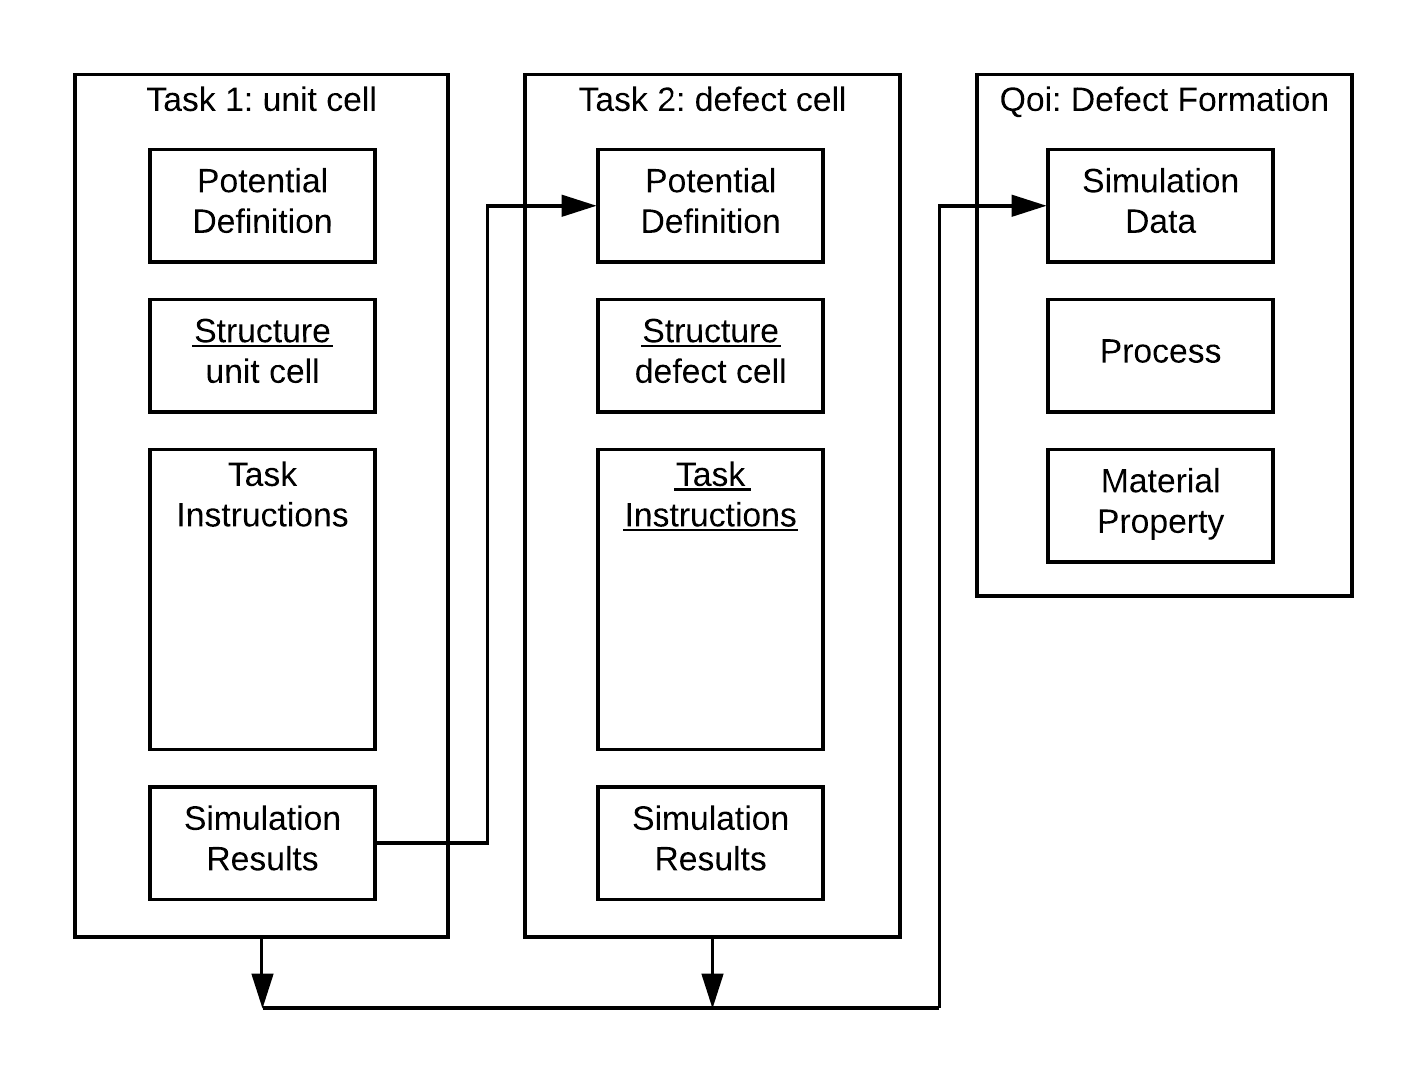
\includegraphics[width=5in]{chapter6/img/fig_point_defect}
	\caption{Schematic for the calculation of point defect calculations.}
\end{figure}

In the first step of the automation process, a potential developer first creates a set of reference simulations required to calculate a material property.  Figure \ref{fig_point_defect_calculation} provides a schematic of various components involved in the calculation of a quantity of interest using the supercell method.  In this case, it starts at a series of LAMMPS or GULP scripts, with the calculation of the material property done with a commercial spreadsheet calculations.

\subsubsection{Simulation Tasks}
\label{sec:pypospack_tasks}

In \emph{pypospack}, the execution of simulation tasks are subclasses of \verb|Task| class.  The derived base classes \verb|LammpsTask| and \verb|GulpTask|, provides the necessary methods for implementing LAMMPS and GULP simulations. \verb|Task| objects are primarily responsible for managing the input and output files for simulation against an external code.  In the expected use of these classes for parameter optimization, an external simulation code is run as a  subprocess to the  \emph{pypospack} application, and derived base classes are reponsible implementing the code for managing these subprocesses.

In the case of LAMMPS simulations, the simulation scripts consists of four sections:  the potential definition, the structure definition, instructions to calculate the required simulation, and an output section.  GULP input scripts can be decomposed in a similar way.

 The \verb|Task| class encapsulates the \verb|Potential| class and the \verb|SimulationCell| class.  As a result, to implement a \verb|Task| class requires three steps: (1) defining of LAMMPS instructions, (2) parsing the output file to retreive the results of the simulation, and (3) populate the \verb|task_results| dictionary with the results.  The first step is already completed in the reference LAMMPS script; the other two steps are rudimentary programming tasks.

The calculation of the Figure \ref{fig_point_defect_calculation} shows material property requires two simulations.  The first simulation involves one involving the minimization of a unit cell representing an ideal bulk structure.  In this simulation, a simulation process known as structural and position relaxation is conducted.  Here, the  minimum of the local energy basin is attained by either steepest descent or conjugate gradient method of minimizing the energy with respect to the atomic positions of each atom, the volume of the simulation cell, and the shape of the supercell.  This simulation provides the energy $E_{c,\mathrm{bulk}}$, as well as structural properties of the lowest energy atomic configuration of the phase represented by the unit cell.  This simulation type has been implemented in as \verb|LammpsStructuralMinimization| and has the \verb|task_type_id| of \verb|min_all|.

The second calculation a simulation involving a defect structure.  Here the defect is embedded into a larger supercell representation of the bulk structure.  This is necessary to prevent defect from interacting with itself across the periodic boundary conditions.  Here the shape and volume of the simulation cell is held fixed, while the conjugate gradient method minimizes the positions only.  This simulation type has been implemented in \verb|LammpsPositionMinimization| and has the \verb|task_type_id| of \verb|min_pos|.

The dependence of the defect calculation upon the results of the  structural properties of the of the ideal bulk is a key feature of this simulation workflow.  \emph{pypospack} solves this problem by aggregating the results of each results of each task into a dictionary object.  Each simulation task is assigned a unique \verb|task_id| which is determined by concatenation of the \verb|structure_id|, \verb|task_type_id|.  For example, if this simulation was done to calculate the vacancy formation energy of silicon, the bulk unit cell might have the name \verb|Si_dia_unit| and the defect structure \verb|Si_dia_vac|.  Then associated \verb|task_ids| would be \verb|Si_dia_unit.min_all| for the minimization of the ideal crystal structure and \verb|Si_dia_vac.min_pos| for the energy calculation of the structure containing the defect.

In the use cases encountered so far, simulations tasks are dependent upon the structural results of their associated bulk structure.  If the \verb|bulk_structure_name| attribute is set on a \verb|Task|, the class will modify the encapsulated \verb|SimulationCell| object after extracting the lattice vectors from the associated structural minimization simulation.  If other dependencies are desired, a new simulation task can be created by subclassing the \verb|LammpsTask| and implement the desired behavior using implemented existing classes as a template.

A simulation task may produce one or more values of intererst.  The simulation produces the cohesive energy $E_c$, and the lattice vectors $\bm{a}_1$, $\bm{a}_1$, and $\bm{a}_3$ of the relaxed structure.  Currently, \emph{pypospack} marshals all simulation results into a dictionary consisting of primitive data types.  As a result, components of the lattice vector $\bm{a}_1$, would have a key values of \verb|a_11|, \verb|a_12|, and \verb|a_13|.

A list of the all the simulation tasks, and a short descriptions are summarized in Table \ref{tbl:pypospack_tasks}.  All simulation task classes are derived from the  \verb|Task| base class. There are two derived base classes: \verb|LammpsTask| and \verb|GulpTask|.

\begin{table}[ht]
	\centering
	\caption{A list of the simulation tasks currently implemented in \emph{pypospack}.}
	\label{tbl:pypospack_tasks}
	\begin{tabular}{ccc}
		\hline
		\verb|task_type_id|
		& Class Name
		& Simulation Engine \\
		\hline
    \verb|min_all|
		& LammpsStructuralMinimization
		& LAMMPS
		\\
		\verb|min_pos|
		& LammpsPositionMinimization
    & LAMMPS
		\\
		\verb|min_none|
		& LammpsStaticCalculation
    & LAMMPS
		\\
		\verb|elastic|,
		& LammpsElasticCalculation
		& LAMMPS
		\\
    \verb|npt|,
		& LammpsNptSimulation
		& LAMMPS
		\\
		\verb|nvt|,
		& LammpsNvtSimulation
		& LAMMPS
		\\
    \verb|gulp_gamma_phonon|
		& GulpGammaPointPhonons
		& GULP
		\\
		\hline
	\end{tabular}
\end{table}

The execution structure for a \verb|Task| happens in stages to accomodate the modification of simulation conditions based on the results of other simulations.  These stages are encoded in the attribute \verb|status|.  The states a \verb|Task| listed in increasing progression: INIT, CONFIG, READY, RUNNING, POST, and FINISHED.  An additional state, ERROR, indicates when there is a problem with the simulation.  Likewise, each status has associated callback methods: \verb|on_INIT|, \verb|on_CONFIG|, \verb|on_READY|, \verb|on_RUNNING|, \verb|on_POST|, AND \verb|on_FINISHED|.  The callback methods can be overridden, but the callback argument signature cannot be changed.  This allows an external procedure to interrogate the status of a class and then provide the necessary information to the class, but defines the process with consistency so that it possible to manage a large number of classes by iterating over a container containing \verb|Tasks|.

This software design supports multiple \verb|Tasks| initialized within a container such as a \verb|list| or \verb|dict|.  The tasks are monitored within a callback loop external to the \verb|Task| objects.  The callback methods of the \verb|Task| objects should be non-blocking so the thread running callback loop can continue to monitor all the simulation tasks.  While \emph{pypospack} is not multi-threaded, multiple simulations are run simulatenously per processor.  Since external simulation codes are run in a child subprocess forked from the \emph{pypospack} process, concurrency issues are the responsibility of the preemptive multi-tasking capabilities of the host operating system.  The callback loop continues until all \verb|Tasks| have either reached a FINISHED or ERROR status.

When an instance of a \verb|Task| is created, the \verb|status| is set to INIT.  A simulation directory with a unique name is created to segregate the file system context of different simulations.  Since external code execution uses an input/output file strategy, it is necessary to provide a unique context to prevent filename conflicts of concurrently running simulations.

The \verb|on_INIT| callback method provides either dictionary necessary to initialize a \verb|Potential| object or an existing \verb|Potential| object is passed by reference.  The secondary mechanism is used to minimize the computational costs of tabulating of EAM potentials into the \emph{setfl} file format.  This process can be demanding especially when the embedding function is determined from inverting an equation of state.  When this task is completed, the \verb|status| attribute is changed from INIT to CONFIG.

the \verb|on_CONFIG| callback method allows the callback loop to provide information which is not available until another simulation is complete.  The results of all completed simulations are passed as a nested dictionary of simulations.  Since each \verb|Task| instance has a unique \verb|task_id|, the task processes the dictionary to identify determine the desired configuration for the simulation.  In our example, the defect calculation awaits the results of the structural relaxation calculation of the bulk system.  If the information is not available, the \verb|status| attribute remains in the INIT state.  When all the necessary configuration information has been acquired, all the necessary input files are written to its simulation directory, and the \verb|status| attribute is changed from CONFIG to READY.

The \verb|on_READY| method encapsulates the \verb|run()| method.  The purpose of this encapsulation is to support multiple methods of task execution.  Support for serial execution of a \verb|Task| is implemented in the \verb|run()| method.  The  location of the external simulation code is determined from the operating system environment variables.  For LAMMPS, the environment variable is \verb|LAMMPS_SERIAL_BIN|.  For GULP, the environment variable is \verb|GULP_SERIAL_BIN|.  These implementation details are encapsulated in the \verb|LammpsTask| and \verb|GulpTask|.  The execution context is changed to its simulation directory, a non-blocking subprocess is created to run the external simulation code, using the Python \verb|subprocess| module to monitor the subprocess.  Some MPI environments, have a default configuration preventing a program from spawn a subprocess, but this can normally be disabled by setting the appropriate MPI environment available in the submission script.  Once the subprocess is created, the \verb|status| attribute is change from READY to RUNNING.

Some \verb|Tasks|,such as NEB calculations, require MPI support.  Other simulations require parallelization in order to complete the simulations in a reasonable amount of time,  NPT and NVT molecular dynamic simulations requiring time integrations are examples.
Since \emph{pypospack} is an MPI-aware application, it is not possible for \emph{pypospack} to subprocess MPI-aware code.  In these cases, the execution of the task is responsibility of an HPC job submission manager, like \emph{pymatgen} implements.  \emph{pypospack} does not implement a persistence model for long-running simulations, but examples to calculate material properties which are dependent upon long-running simulations is provided in the distribution.

The \verb|on_RUNNING| polls the external simulation code.  Here there are a variety of techniques used to identify a simulation failure.  First, the \verb|subprocess| module allows us to check is the application is running, exited normally, or exited with an error.  If the external simulation code exited with an error, then the attribute \verb|status| is marked ERROR.    If the application is running, the \verb|Task| will check to see how long the simulation is running. If the total time of the simulation exceeds \verb|max_simulation_time|, a variety of process management steps are applied to kill the child process without interrupting the parent process.  When the subprocess is terminated, the \verb|status| is marked ERROR.  If the simulation code exited normally, the attribute \verb|status| is marked POST, indicating the simulation is complete.

The \verb|on_POST| method instructs the task to parse the output files from the external simulation code and populate a dictionary containing the results of the simulation.  The attributes of the simulation both returned to the callback thread and set as the attribute value \verb|results|.  After the post-simulation activities have been completed, the \verb|status| attribute is sent to FINISHED.

This approach to software development minimizing the software development expertise required to contribute to \emph{pypospack}'s capabilities by developing new simulation tasks and calculation of material properties by by providing a well-defined process to convert an existing LAMMPS script into an automatable simulation task.

\subsubsection{Material Properties}

The material properties are referred to more generally in the software by the term quantity of interest (QOI), a term coming from  from verification, validation, and uncertainty quantification (VVUQ) literature.
The calculation of material properties is implemented as subclasses of the \verb|Qoi| base class.

Since an identical set of simulations can be used to calculate one or more material properties, a \verb|Qoi| class may implement the calculation of one or more material properties.  However, a potential developer may not be interested in optimizing to all these material properties.  Each implemented \verb|Qoi| class must implement a static \verb|qoi_names| attribute.  This attribute is a list of strings, which identify which material property which is modelled by the implemented \verb|Qoi| subclass.  This enables the construction of a lookup table which correlates the QOI name string to its implementing \verb|Qoi| class through introspection, providing the many to one mapping.

Like \verb|Task| classes, \verb|Qoi| classes to be accessed in a container holding multiple \verb|Qoi| objects with identical interfaces.  To prevent multiple instancing of a \verb|Qoi| class, it is necessary to provide a unique identifier, \verb|qoi_id|, fo each instance.

In single structure simulations, the naming convention is simple.  The \verb|structure_id| of the structure is joined with the \verb|qoi_type_id|  For example, both the calculation of the cohesive energy of structure  and the magnitude of the $\bm{a}_1$ lattice vector map onto the same class.  If the \verb|structure_id| was \verb|Ni_fcc_unit|.  The first request would instantiate a class \verb|RelaxedStructureCalculations| with a unique \verb|qoi_id|, \verb|Ni_fcc_unit.lmps_min_all|.  The second request would provide an identical \verb|qoi_id| preventing a second instantiation.  For retrieval of the individual properties, the cohesive energy is contained in the \verb|E_cohesive| entry of the \verb|results| dictionary, while the the magnitude of the $\bm{a}_1$ lattice vector would be contained as an \verb|a1| entry.

Some material property calculations are dependent upon more than two calculations.  An automatic \verb|qoi_id| is generated by joining the \verb|structure_id| of the characteristic structure, the \verb|qoi_type_id| of the implemented \verb|Qoi| class.  For example, a surface energy calculation is dependent upon the simulations of a slab structure and the bulk structure.  Only the slab structure calculation is characteristic of the calculation; the bulk structure calculation is a reference calculation.  The \verb|qoi_id| for a surface energy calculation, is \verb|E_surface_energy| which \emph{pypospack} locates the \verb|SurfaceEnergyCalculation| implementing class.  If the \verb|structure_id| of the slab structure is \verb|Ni_fcc_s100|, then the \verb|qoi_id| of this instance of \verb|SurfaceEnergyCalculation| is \verb|Ni_fcc_s100.lmps_surface_energy|.  A list of the currently implemented classes in contained in Table \ref{tbl:pypospack_qoi_classes}.

\begin{table}[ht]
	\centering
	\caption{A list of the Qoi classes}
	\label{tbl:pypospack_qoi_classes}
	\begin{tabular}{cc}
		\hline
		Class Name
		  & \verb|qoi_type_id| \\
		\hline
    GulpOptiCalculations
		   & \verb|gulp_opti_calc| \\
		StaticStructureCalculations
		   & \verb|lmps_min_none| \\
		RelaxedPositionCalculations
		   & \verb|lmps_min_pos| \\
		RelaxedStructureCalculations
		   & \verb|lmps_min_all| \\
    ElasticPropertyCalculations
		   & \verb|lmps_elastic| \\
		PhaseOrderCalculation
		   & \verb|phase_order| \\
		DefectFormationEnergy
		   & \verb|lmps_defect| \\
		SurfaceEnergyCalculation
		   & \verb|lmps_surface_energy|  \\
		StackingFaultEnergyCalculation
			 & \verb|lmps_stacking_fault| \\
		ThermalExpansion
			 & \verb|lmps_thermal_expansion| \\
		\hline
	\end{tabular}
\end{table}


For material property calculations that have two characteristic structures, such as the energy difference between two phases, both of the characteristic structures are included in the prefix.  For example, the phase energy difference between \verb|Ni_fcc_unit| and \verb|Ni_bcc_unit| the prefix string would be \verb|Ni_fcc_unit__Ni_bcc_unit|.

The implementation of a \verb|Qoi| class is simple.  The declaration of static class variables \verb|qoi_type_id| and \verb|qoi_names| is necessary so that introspection code can create the necessary mappings.   The default constructor needs to accept the following arguments: \verb|qoi_name|, \verb|qoi_type|, and \verb|structures|.   The first two arguments give the software developer the option override the default naming conventions.  The \verb|structures| argument is a \verb|dict| argument containing identifying the necessary structures.  For the calculation of a surface energy, the \verb|structure| dictionary would expect to have two entries; a \verb|slab| key entry providing the \verb|structure_id| of the slab structure, and a \verb|bulk| key entry of the \verb|structure_id| for the ideal bulk.

To determine determine which simulations need to be completed, the method \verb|determine_tasks| needs to be implemented.  To prevent duplication of simulations, the \verb|task_id| is also unique.  For example, the calculation of all defect calculations are dependent upon the structural minimization of the bulk structure.  The \verb|task_id| of these simulations are identical (e.g. \verb|Ni_fcc_unit.min_all|), which allows the instantiating code from executing duplicated identical simulations.  The class stores the \verb|task_id| for the simulations it requests, and returns a nested dictionary providing the necessary configuration for each \verb|Task| which needs to be instantiated.

When the simulation tasks have been completed, a nested dictionary containing all the \verb|Task| simulation results is send to the \verb|process_task_results| method.  The class then makes a local copy of specific simulation results that it needs.  This functionality is implemented by the \verb|Qoi| base class.

To calculate the QOIs supported by a \verb|Qoi| the \verb|calculat_qoi_class| verb needs to be implemented.  Since the results of the requested simulation tasks are stored in the \verb|task_results|, the simulations results can then be used to calculate the material properties which is implemented by the \verb|Qoi| subclass.

A variety of \verb|Qoi| class have already been implmented.  Material properties structure calculated by a single structure are implemented by
the \verb|GulpOptiCalculations|
    (see Table \ref{tbl:pypospack_qoi_gulp_opti} ),
the \verb|StaticStructureCalculations|
    (see Table \ref{tbl:pypospack_qoi_lmps_min_none}),
the \verb|RelaxedPositionCalculations|
    (see Table \ref{tbl:pypospack_qoi_lmps_min_pos}),
the \verb|RelaxedStructureCalculations|
    (see Table \ref{tbl:pypospack_qoi_lmps_min_all}),
and the \verb|ElasticPropertyCalculations|
    (see Table \ref{tbl:pypospack_qoi_lmps_elastic})
		classes.
Material properties calculated from multiple structures are implemented by
\verb|PhaseOrderCalculation|
    (see Table \ref{tbl:pypospack_qoi_lmps_phase_order}),
\verb|DefectFormationEnergy|
    (see Table \ref{tbl:pypospack_qoi_lmps_defect}),
\verb|SurfaceEnergyCalculation|
    (see Table \ref{tbl:pypospack_qoi_lmps_surface_energy}), and
\verb|StackingFaultEnergyCalculation|
    (see Table
		    \ref{tbl:pypospack_qoi_lmps_stacking_fault}) classes.
The \verb|ThermalExpansion| class to calculate thermal expansion from a series of NPT simulations is implemented, but since these simulations are long running, they would not be typically be used in parameter optimization.

\begin{table}[ht]
	\centering
	\caption{Material properties available from GULP calculations after structural minimization implemented in the class \emph{GulpOptiCalculations}}
	\label{tbl:pypospack_qoi_gulp_opti}
	\begin{tabular}{ccc}
		\hline
		QOI name & Units & Description \\
		\hline
		\verb|Ecoh_min_all_g|
		    & eV/atom
				& Cohesive energy\\
    \verb|a11_min_all_g|
		    & \AA
				& $a_{11}$ component of the $\bm{a}_1$ lattice vector \\
	  \verb|a12_min_all_g|
		    & \AA
				& $a_{12}$ component of the $\bm{a}_1$ lattice vector \\
	  \verb|a13_min_all_g|
		    & \AA
				& $a_{13}$ component of the $\bm{a}_1$ lattice vector \\
    \verb|a21_min_all_g|
		    & \AA
				& $a_{21}$ component of the $\bm{a}_2$ lattice vector\\
	  \verb|a22_min_all_g|
		    & \AA
				& $a_{22}$ component of the $\bm{a}_2$ lattice vector \\
	  \verb|a23_min_all_g|
		    & \AA
				& $a_{23}$ component of the $\bm{a}_2$ lattice vector \\
    \verb|a31_min_all_g|
		    & \AA
				& $a_{31}$ component of the $\bm{a}_3$ lattice vector \\
	  \verb|a32_min_all_g|
		    & \AA
				& $a_{32}$ component of the $\bm{a}_3$ lattice vector \\
	  \verb|a33_min_all_g|
		    & \AA
				& $a_{33}$ component of the $\bm{a}_3$ lattice vector \\
		\hline
	\end{tabular}
\end{table}

\begin{table}[ht]
	\centering
	\caption{Materials properties available in the QOI class \emph{StaticStructureCalculations}}
	\label{tbl:pypospack_qoi_lmps_min_none}
	\begin{tabular}{ccc}
		\hline
		QOI name & Units & Description \\
		\hline
	  \verb|Ecoh_min_none|
			& eV/atom
			& Cohesive energy\\
    \verb|a1_min_none|
		  & \AA
			& Magnitude of the $\bm{a}_1$ lattice vector \\
		\verb|a2_min_none|
			& \AA
			& Magnitude of the $\bm{a}_2$ lattice vector \\
		\verb|a3_min_none|
			& \AA
			& Magnitude of the $\bm{a}_2$ lattice vector \\
    \verb|a11_min_none|
			& \AA
			& $a_{11}$ component of the $\bm{a}_3$ lattice vector \\
		\verb|a12_min_none|
			& \AA
			& $a_{12}$ component of the $\bm{a}_3$ lattice vector \\
		\verb|a13_min_none|
			& \AA
			& $a_{13}$ component of the $\bm{a}_3$ lattice vector \\
    \verb|a21_min_none|
			& \AA
			& $a_{21}$ component of the $\bm{a}_3$ lattice vector \\
		\verb|a22_min_none|
			& \AA
			& $a_{22}$ component of the $\bm{a}_3$ lattice vector \\
		\verb|a23_min_none|
			& \AA
			& $a_{23}$ component of the $\bm{a}_3$ lattice vector \\
		\verb|a31_min_none|
			& \AA
			& $a_{31}$ component of the $\bm{a}_3$ lattice vector \\
		\verb|a32_min_none|
			& \AA
			& $a_{32}$ component of the $\bm{a}_3$ lattice vector \\
		\verb|a33_min_none|
			& \AA
			& $a_{33}$ component of the $\bm{a}_3$ lattice vector \\
		\verb|p_11_min_none|
			& bar
			& $P_{11}$ component of the pressure tensor \\
		\verb|p_12_min_none|
			& bar
			& $P_{12}$ component of the pressure tensor \\
		\verb|p_13_min_none|
			& bar
			& $P_{13}$ component of the pressure tensor \\
		\verb|p_21_min_none|
			& bar
			& $P_{21}$ component of the pressure tensor \\
		\verb|p_22_min_none|
			& bar
			& $P_{22}$ component of the pressure tensor \\
		\verb|p_23_min_none|
			& bar
			& $P_{23}$ component of the pressure tensor \\
    \verb|p_31_min_none|
		  & bar
			& $P_{31}$ component of the pressure tensor \\
		\verb|p_32_min_none|
			& bar
			& $P_{32}$ component of the pressure tensor \\
		\verb|p_33_min_none|
			& bar
			& $P_{33}$ component of the pressure tensor \\
		\hline
	\end{tabular}
\end{table}

\begin{table}[ht]
	\centering
	\caption{Materials properties available in the QOI class \emph{RelaxedPositionCalculations}}
	\label{tbl:pypospack_qoi_lmps_min_pos}
	\begin{tabular}{ccc}
		\hline
		QOI name & description \\
		\hline
		\verb|Ecoh_min_pos|
			& eV/atom
			& Cohesive energy\\
    \verb|a1_min_pos|
		  & \AA
			& Magnitude of the $\bm{a}_1$ lattice vector \\
		\verb|a2_min_pos|
			& \AA
			& Magnitude of the $\bm{a}_2$ lattice vector \\
		\verb|a3_min_pos|
			& \AA
			& Magnitude of the $\bm{a}_2$ lattice vector \\
    \verb|a11_min_pos|
			& \AA
			& $a_{11}$ component of the $\bm{a}_3$ lattice vector \\
		\verb|a12_min_pos|
			& \AA
			& $a_{12}$ component of the $\bm{a}_3$ lattice vector \\
		\verb|a13_min_pos|
			& \AA
			& $a_{13}$ component of the $\bm{a}_3$ lattice vector \\
    \verb|a21_min_pos|
			& \AA
			& $a_{21}$ component of the $\bm{a}_3$ lattice vector \\
		\verb|a22_min_pos|
			& \AA
			& $a_{22}$ component of the $\bm{a}_3$ lattice vector \\
		\verb|a23_min_pos|
			& \AA
			& $a_{23}$ component of the $\bm{a}_3$ lattice vector \\
		\hline
	\end{tabular}
\end{table}

\begin{table}[ht]
	\centering
	\caption{Materials properties available in the QOI class \emph{RelaxedStructureCalculations}}
	\label{tbl:pypospack_qoi_lmps_min_all}
	\begin{tabular}{ccc}
		\hline
		QOI name & Units & Description \\
		\verb|Ecoh_min_pos|
			& eV/atom
			& Cohesive energy\\
		\verb|a1_min_pos|
			& \AA
			& Magnitude of the $\bm{a}_1$ lattice vector \\
		\verb|a2_min_pos|
			& \AA
			& Magnitude of the $\bm{a}_2$ lattice vector \\
		\verb|a3_min_pos|
			& \AA
			& Magnitude of the $\bm{a}_2$ lattice vector \\
		\verb|a11_min_pos|
			& \AA
			& $a_{11}$ component of the $\bm{a}_3$ lattice vector \\
		\verb|a12_min_pos|
			& \AA
			& $a_{12}$ component of the $\bm{a}_3$ lattice vector \\
		\verb|a13_min_pos|
			& \AA
			& $a_{13}$ component of the $\bm{a}_3$ lattice vector \\
		\verb|a21_min_pos|
			& \AA
			& $a_{21}$ component of the $\bm{a}_3$ lattice vector \\
		\verb|a22_min_pos|
			& \AA
			& $a_{22}$ component of the $\bm{a}_3$ lattice vector \\
		\verb|a23_min_pos|
			& \AA
			& $a_{23}$ component of the $\bm{a}_3$ lattice vector \\
		\hline
	\end{tabular}
\end{table}

\begin{table}[ht]
	\centering
	\caption{Materials properties available in the QOI class \emph{ElasticPropertyCalculations}}
	\label{tbl:pypospack_qoi_lmps_elastic}
	\begin{tabular}{ccc}
		\hline
		QOI name & Units &description \\
		\hline
		\verb|c11|
		  & GPa
		  & $C_{11}$ component of the elastic tensor\\
		\verb|c12|
		  & GPa
		  & $C_{12}$ component of the elastic tensor\\
		\verb|c13|
		  & GPa
		  & $C_{13}$ component of the elastic tensor \\
		\verb|c22|
		  & GPa
			& $C_{22}$ component of the elastic tensor \\
		\verb|c23|
			& GPa
			& $C_{23}$ component of the elastic tensor \\
		\verb|c33|
			& GPa
			& $C_{22}$ component of the elastic tensor \\
		\verb|c44|
			& GPa
			& $C_{44}$ component of the elastic tensor \\
		\verb|c55|
			& GPa
			& $C_{55}$ component of the elastic tensor \\
		\verb|c66|
			& GPa
			& $C_{66}$ component of the elastic tensor \\
		\verb|bulk_modulus|
			& GPa
			& Bulk modulus \\
		\verb|shear_modulus|
			& GPa
			& Sheer modulus \\
		\hline
	\end{tabular}
\end{table}

\begin{table}[ht]
	\centering
	\caption{Materials properties available in the QOI class \emph{PhaseOrderCalculation}}
	\label{tbl:pypospack_qoi_lmps_phase_order}
	\begin{tabular}{ccc}
		\hline
		QOI name & Units & Description \\
		\hline
		\verb|phase_order|
		  & eV
			& The energy difference between two competing phases\\
		\hline
	\end{tabular}
\end{table}

\begin{table}[ht]
	\centering
	\caption{DefectFormationEnergy}
	\label{tbl:pypospack_qoi_lmps_defect}
	\begin{tabular}{ccc}
		\hline
		QOI name & units & Description \\
		\hline
		\verb|E_formation|
		 	& eV
			& Defect formation energy\\
		\hline
	\end{tabular}
\end{table}

\begin{table}[ht]
	\centering
	\caption{Materials properties available in QOI class \emph{SurfaceEnergyCalculation}}
	\label{tbl:pypospack_qoi_lmps_surface_energy}
	\begin{tabular}{ccc}
		\hline
		QOI name & Units & Description \\
		\hline
		\verb|E_surface|
		  & eV/$\text{\AA}^2$
			& Surface energy \\
		\hline
	\end{tabular}
\end{table}

\begin{table}[ht]
	\centering
	\caption{Materials properties available in \emph{StackingFaultEnergyCalculation}}
	\label{tbl:pypospack_qoi_lmps_stacking_fault}
	\begin{tabular}{ccc}
		\hline
		QOI name & Units & Description \\
		\hline
		\verb|E_stacking_fault|
		& eV/$\text{\AA}^2$
		& Surface energy \\
		\hline
	\end{tabular}
\end{table}

\subsubsection{Coordination Framework}

In parameter optimization, a potential developer is likely interested in evaluating a large number material properties, from which an even larger number of simulation tasks are generated.

Up to this point, classes have been segregated in functionality.  The \verb|Potential|, \verb|SimulationCell|, \verb|Task|, and \verb|Qoi| classes are decoupled.  All the components to define various components to evaluate a set of parameters, $\bm{\theta}$, have been defined.  However, we do not have an initialization and execution framework.
\begin{figure}[ht]
	\label{fig:pypospack_coordination}
	\centering
	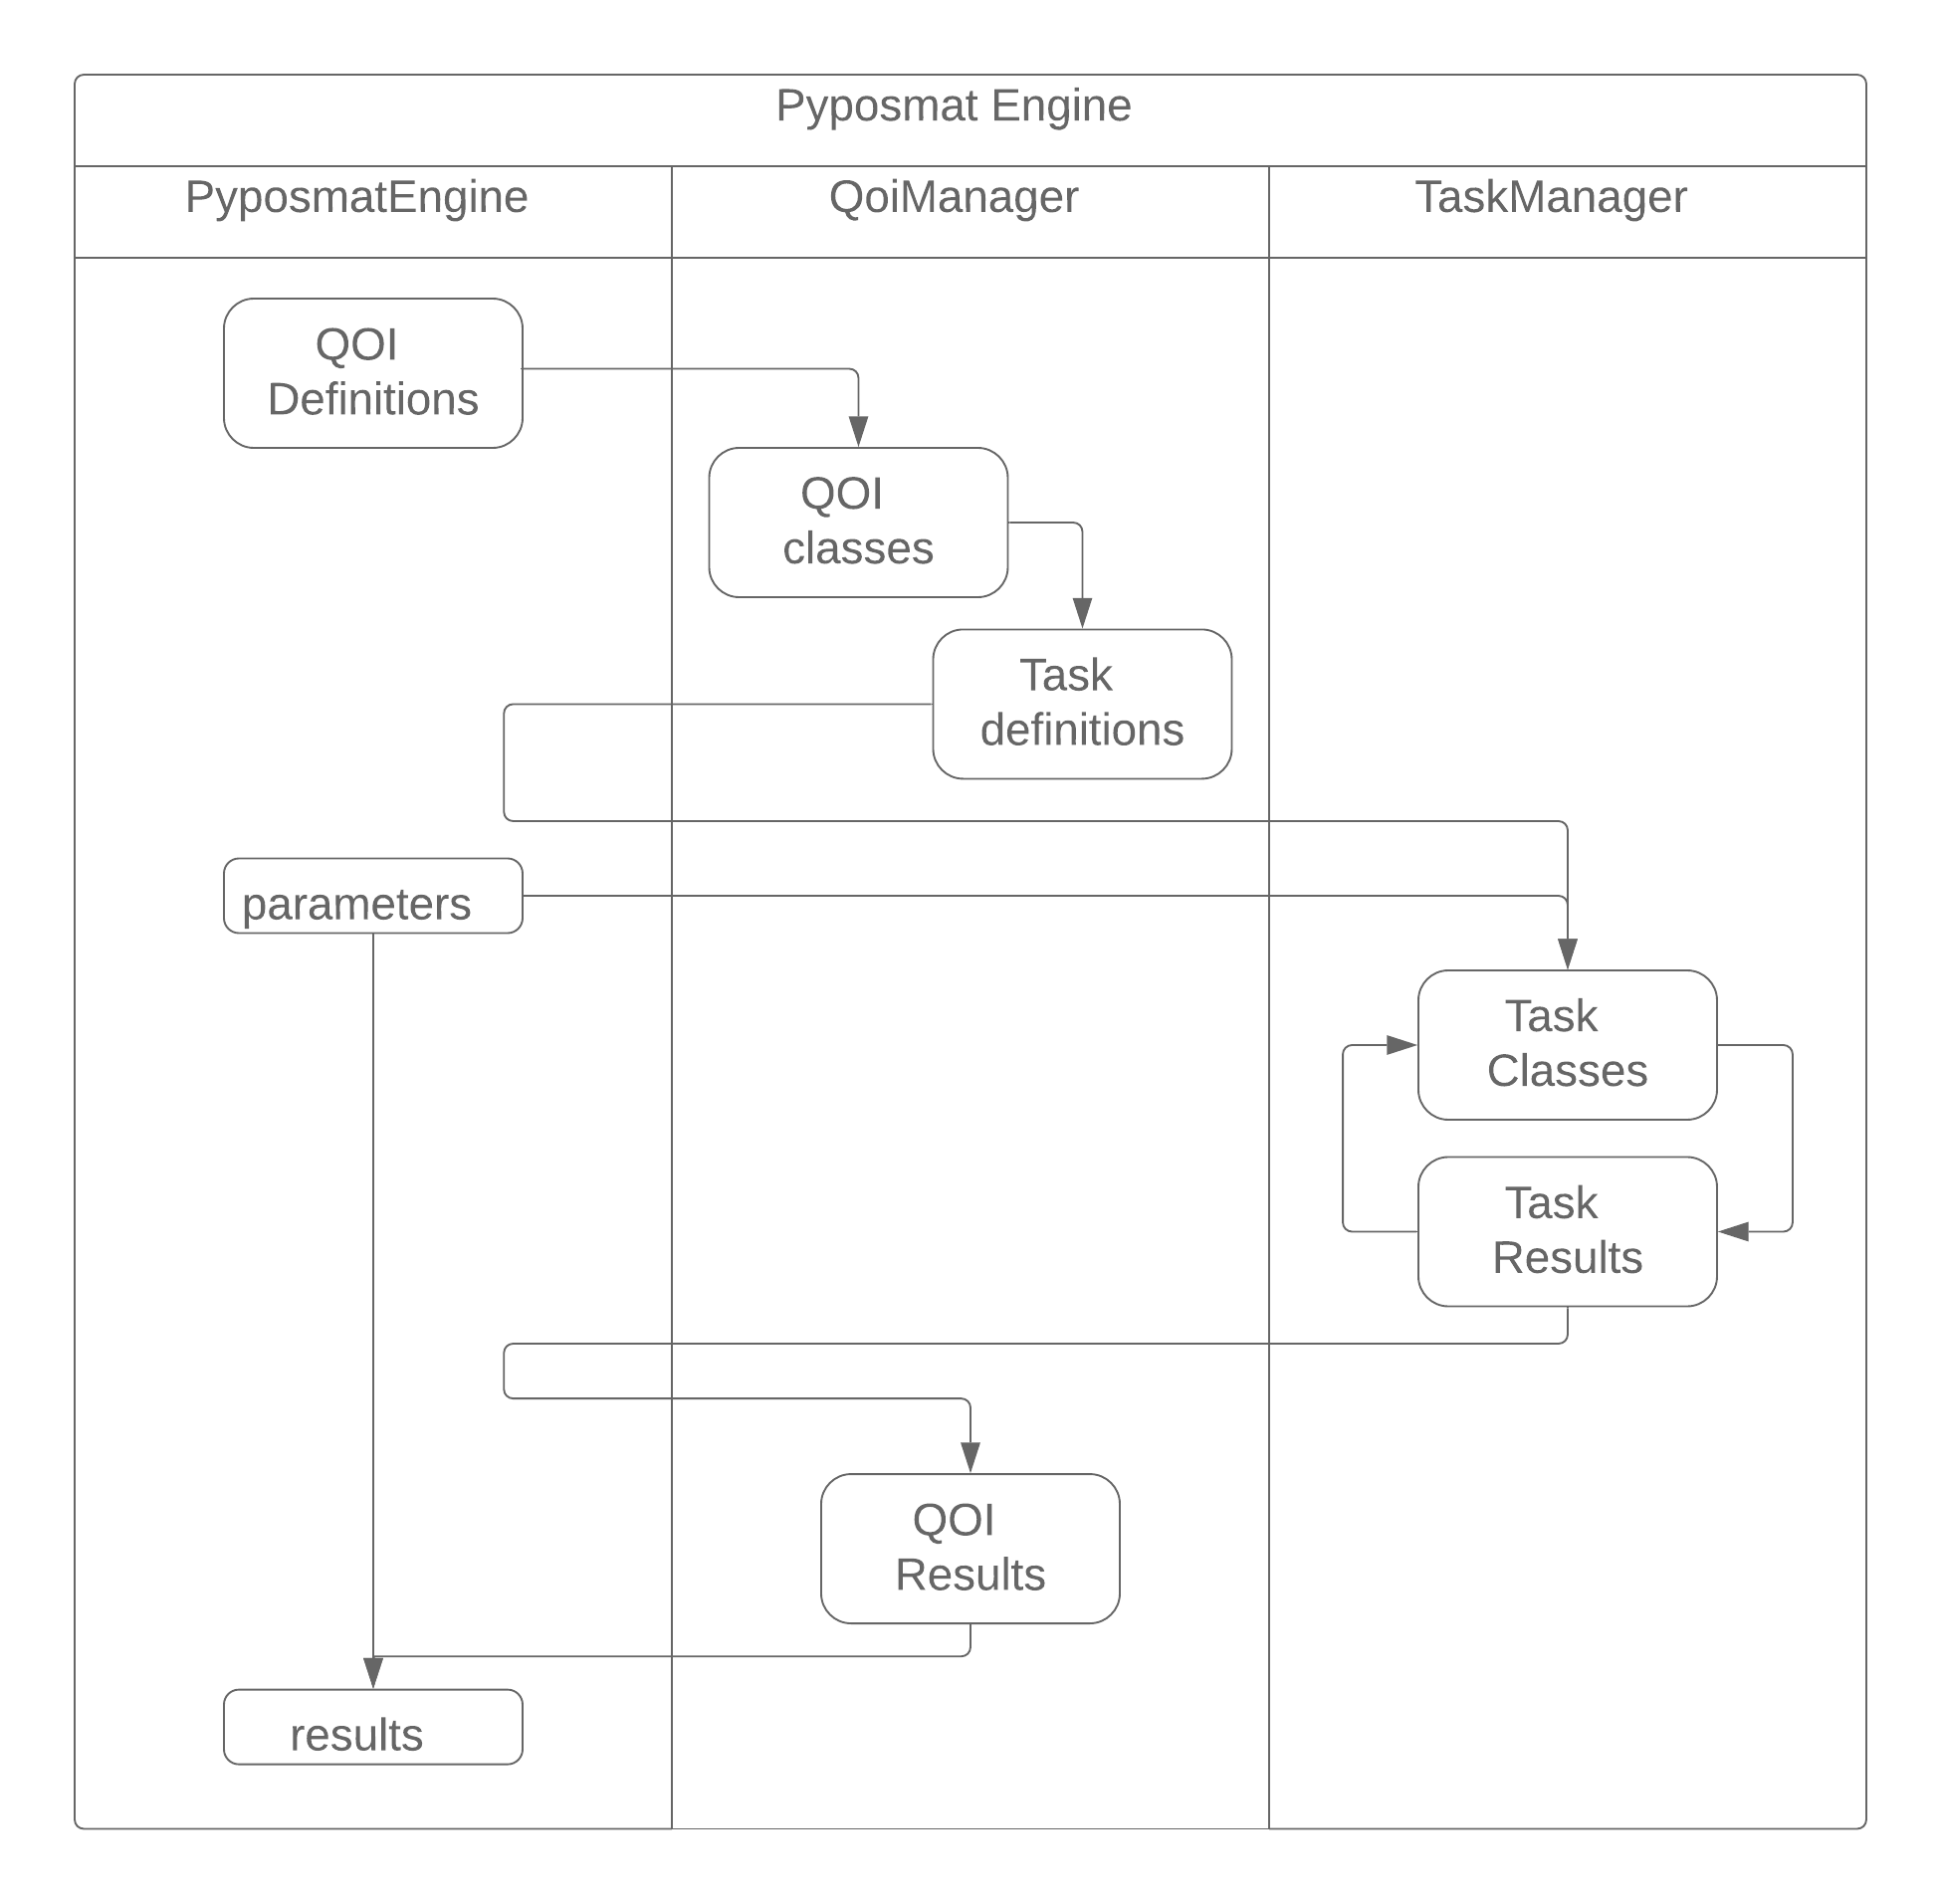
\includegraphics[width=5in]{chapter6/img/pypospack_coordination}
	\caption{Schematic of for the calculation of point defect calculations.}
\end{figure}

While the base classes are designed to support more scalable concurrency schemes, such parallelization over tasks, these core classes are combined in the \verb|pyposmat| module which minimizes the concurrency issues with parameter evaluation by serial execution of the simulation tasks on a single processor.

\verb|PyposmatEngine| encapsulates three objects: \verb|PyposmatConfigurationFile|, \verb|QoiManager|, and \verb|TaskManager|.
\verb|QoiManager| and \verb|TaskManager| are containers for the large numbers \verb|Qoi| classes and \verb|Task| classes generated.    \verb|PyposmatEngine| is a class which coordinates the information flows.

The execution of a parameter set will be described procedurally.  Figure \ref{fig:pypospack_coordination} is a swimlane schematic that diagrams the information flows in the calculation of a material property.

The \verb|PyposmatConfigurationFile| is a collection of dictionaries, which provides the configuration the potential formalism, the structure database, and descriptors of the material properties with their associated target values.
The \verb|PyposmatConfigurationFile| read and writes YAML formatted files which are stored internally are a series of dictionary objects.
Instead of a proprietary input file, \emph{pyposmat} applications are configured from defining a series of dictionary objects to instantiate a \verb|PyposmatConfigurationFile|.
Since the configuration of a \emph{pyposmat} application is supported by simple dictionary objects with the fully-featured langauge support of Python, complex workflows can be quickly evolved starting from simple simulations.
Since dictionary objects are easily serializable/deserializable to YAML, the \emph{pyposmat} application can be configured completely from a YAML file.

The \verb|PyposmatEngine| class can either be instantiated from a YAML formatted file, a dictionary object, or by passing an instance \verb|PyposmatConfigurationFile| to the default constructor.  To support multiple \verb|PyposmatEngine| instances running simultaneously, filesystem path can be provided to ensure that each instance has a unique context so that the input and output files generated by the simulation tasks do not conflict with each other.

From the \verb|PyposmatConfigurationFile|, the descriptors necessary to configure the \verb|Qoi| objects are passed to the \verb|QoiManager|, which then instantiates all the \verb|Qoi| classes into a container.  When this is complete, \verb|PyposmatEngine| then receives all the descriptors for each simulation task from the \verb|QoiManager| which iterates over \verb|Qoi|, and eliminating identical tasks.

\verb|PyposmatEngine| then instantiates \verb|TaskManager| and provides it with the \verb|Task| descriptors.  Using these descriptors, \verb|TaskManager| now instantiates each \verb|Task| within a common container.  Since each \verb|Task| is now has an INIT stats, each \verb|Task| needs a requires a potential definition.  \verb|PypospackEngine| transfers this information from the configuration information, to the \verb|TaskManager| which iterates over all \verb|Task| objects, providing the potential formalism information, which causes all \verb|Tasks| to move to the CONFIG state.

In the next step, a parameter set is sent to the \verb|TaskManager| for evaluation.  The \verb|TaskManager| now creates the necessary  callback thread described in Section \ref{sec:pypospack_tasks}.  First, where it queries the status of each \verb|Task| and calls the appropriate callback method.  This allows \verb|TaskManager| to provide the dictionary containing the aggregated \verb|task_results| and the parameter set to be evaluated when necessary.  When any of the \verb|Tasks| has an ERROR state, a \verb|PyposmatBadParameterError| is propagated, terminating the evaluation process.  This allows \emph{pyposmat} applications to handle failures of external simulation codes.  When all \verb|Tasks| reach the FINISHED state, \verb|TaskManager| terminates the callback loop, and returns the aggregated \verb|task_results|.

\verb|PyposmatEngine| now provides \verb|task_results| to the \verb|QoiManager|, which distributes the results to each \verb|Qoi| class, instructs each class to calculate the predicted material properties ($\hat{q}_i(\bm{\theta})$), and difference between the predicted material properties and the target values ($\epsilon_i = \hat{q}_i(\bm{\theta})-q_i$).

\section{Sampling Strategies}
\label{sec:software_sampling_strategies}

The algorithm described in Chapter \ref{ch:methodology} demands thousands of parameters to be sampled, while \verb|PypospackEngine| samples evaluates a single given parameter.  This algorithm evolves an an initial probability distribution, $p_{\bm{Theta}}(\bm{\theta})$, so that we can generate samples from a random variable $\bm{\theta}(\omega) \in \bm{\Theta}(\Omega)$ with $\omega \in \Omega$.

This process is abstracted into four components: sampler clases, filtering classes, analysis classes, and an iterative sampler class.  Sampler class implement a sampling strategy which generates $\bm{\theta}$, evaluates

Sampler classes are subclasses of the \verb|PyposmatSampler| base class, which itself is a subclass of \verb|PyposmatEngine|.  There are five \emph{pyposmat} sampling strategies and they are listed in \ref{tbl:pyposmat_samplers} with their associated \verb|sampling_type_id|.  With the exception of the \verb|FileSampler|, sampling is by drawing random variates from a probability distribution, as described in Chapter \ref{ch:probability}, utilizing the probability libraries of SciPy.

\begin{table}[ht]
	\centering
	\caption{A list of the different sampling strategies and their implementing class}
	\label{tbl:pyposmat_samplers}
	\begin{tabular}{cc}
		\hline
		\verb|sampling_type_id| & Class Name \\
		\hline
		\verb|parametric| & UnivariateSampler \\
		\verb|kde| & KdeSampler \\
		\verb|mvn| & MultivariateNormalSampler \\
		\verb|from_from| & FileSampler \\
		\verb|kde_cluster| & KdeClusterSampler \\
		\hline
	\end{tabular}
\end{table}

The \verb|UnivariateSampler| treats each each parameter as an independent random variate described by its own univariate probability density function.  This class is used in the first iteration in the parameter estimation process described in Chapter \ref{ch:methodology} as an initial distribution.  Since the univariate sampler uses parametric distributions, for each free \emph{potential parameter}, the probability distribution function must be fully specified by providing the probability distribution type and the parameters of the probability distribution function.  The \verb|UnivariateSampler| implements the uniform and normal probability density functions, which must be provided as a dictionary object to the class.

The \verb|KdeSampler| enables sampling from a kernel density estimate (KDE) as a non-parametric probability density representation of the Pareto set.  The \verb|KdeSampler| implements the automatic determination of the bandwidth parameter using Scott, Silverman, and Chiu.  The Chiu estimator is a cross-validation bandwidth estimator, which is superior when the number of candidate potentials are small ($N<1000$), but as the number of candidate potentials increases becomes computationally inefficient due to the nature of estimation with cross-validation methods.  The \verb|KdeSampler| is defined by the potential parameters of all the candidates; the path of the location of a \verb|PyposmatDataFile| must be provided to the \verb|KdeSampler|.

The \verb|MultivariateNormalSampler| enables sampling from the multivariate normal distribution, described by $\bm{\mu}$ and $\bm{Sigma}$. $\bm{\mu}$ is a vector of the means of the potential parameters. $\bm{\Sigma}$ is the variance covariance matrix of the potential parameters.  The class can be used by providing the path of a \verb|PyposmatDataFile| which will use the descriptive statistics of the population of candidate potentials.
Alternately, \verb|mu| and \verb|sigma| can be provided either through the \verb|PyposmatConfigurationFile| or directly.

To implement equality potential parameter constraints, \emph{pypospack} removes potential parameters bound by equality constraints, and only generates potential parameters free of equality constraints.  The enforcement of equality constraints occurs by direct calculation of the potential parameters.  Inequality constraints on the potential parameters is enforced by rejecting generated potential parameters set which fail any inequality constraint.  A \emph{PyposmatBadParameterError} exception is raised and the offending parameter set is recorded in a bad parameters file.

Both the \verb|KdeSampler| and \verb|MultivariateNormalSampler| are dependent upon the Cholesky decomposition of the covariance matrix.  While all covariance matrices are by definition positive definite, these matrices can be ill-conditioned.
In these cases, \emph{pypospack} will modify the variance-covariance matrix by eigendecomposition, and set negative eigenvalues to a small positive number, and then use the modified covariance matrix.
This modification makes the covariance matrix positive-definite by definition and slightly biases the orientation of the covariance matrix in the direction of the least influential eigenvector.

\section{Analyzing Simulations}
\label{sec:pypospack_analyze}
At the end of the simulations, there are typically thousands of simulations to analyze.  In order to evolve distribution, it is necessary remove the results which are undesireable.  In the \emph{pyposmat} application, this process is referred to as filtering.  A series of filters is defined and applied to the dataset.  Each filter is independent upon each other, and provides a list of surviving candidate potentials.  The union of the surviving candidate potentials from each filter operation can then be applied to define the KDE for the next sampling iteration.  Three filtering operations have been implemented in \emph{pyposmat}: (1) the Pareto filter, (2) the performance constraint filter, and the (3) the scoring filter.

The Pareto filter removes the dominated potentials from the list of candidate potentials.  Determining the Pareto set is a compuationally expensive operation which increases with the number of candidates.  To speed the cost of computation, \emph{pyposmat} takes advantage that the majority of the potentials are dominated.  \emph{pyposmat} partitions the potential list into smaller subsets and removes the Pareto dominated points.  The non-dominated points from each partition are then concatenated, then updated candidate potentials are repartition into subsets switch have twice the number of candidates as the previous iteration.  This process is continued until the Pareto set is obtained.

The second type of filtering operation is the enforcement of the peformance constraints defined at the beginning of the parameter optimization process.  \emph{pyposmat} only supports inequality constraints.  In addition to static performance constraints, dynamic univariate constraints that eliminates the worst performing potentials on a percentile basis.

The final filter is a flexible scoring filter.  This filter allows the definition of a scoring function which can either keep a static number of potentials.  The purpose of this filter is to eliminate potentials with pathologically poor performance.  The scoring function can either be the sum or the sumproduct of weighted loss functions.  The absolute error and square error functions have been implemented, and a variety of weighting schemes have been implemented.  By default, the errors are rescaled by the magnitude of the target values, the errors are then squared and summed.  This correspond to the potentials closest to the origin.

The process for analysis in the included \emph{pyposmat} application is to remove to apply a variety of filters.

\subsection{Convergence}

The Kullback-Leiber diverence is calculated on the parameters of the filter parameters from the current iteration and the previous iteration.  Due to problems with ill-conditioned covariance matrices, this metric is not implemented as a stopping condition, but is calculated to determine if the probability distribution is sufficiently converged.

\subsection{Clustering}

The probability distribution of the Pareto optimal parameter set displays heteroskedacity; there are sub-populations that have different covariance matrix from others.  The KDE applies a bandwidth smoothing factor to a static covariance distribution. this implies that the orientation of the covariance matrix.  To overcome these problems, \emph{pypospack} has support for the classification algorithm identified the machine learning package \emph{scikit-learn}.

Two clustering algorithms have been implemented.  The first technique combines a manifold learning technique and then applies a clustering algorithm.  The second technique implements a Gaussian mixture model.  Each technique has three options: the identification of  clusters based upon the distribution of parameters, the identification of clusters based upon the potentials predicted estimates of each QOI, and identification of clusters by treating both parameter and performance space together.  The purpose of the third option is to ensure that clusters in parameter space are also sufficiently close together in performance space.

Running the cluster algorithm produces a new column in the datafile \verb|cluster_id|, which assigns each potential to a specific cluster.  When this file is passed to the \verb|KdeClusterSampler|, the total number of simulations is divided among the number of clusters.  Since cluster is sampled with it's own KDE based upon its members, the orientation of the covariance matrix is specific to each cluster.

\section{Iterative Improvement}
	\label{sec:pypospack_iteration}

The \verb|PyposmatIterativeSampler| encapsulates the \verb|PyposmatSamplers|, filtering rules, and analysis routines discussed in the previous section.  For configuration, a nested dictionary containing the configuration of each iteration must be provided.  The configuration of the first iteration defines the intial starting conditions, either by using the \verb|UnivariateSampler| to express a non-informative distribution or the \verb|FileSampler| if starting from a pre-converged set of points.   The following iterations uses  the \verb|KdeSampler| to define the KDE from the filtered results of the previous iteration.

The \verb|PyposmatIterativeSampler| implements parrellization schemes to allow \emph{pyposmat} to use many processors in HPC environments.  In \emph{ab initio} workflow management schemes, simulation tasks are sent to the HPC job manager, such as SLURM, and the workflow manager polls SLURM to identify when simulations are complete.  In our computational problem, our applications evaluates tens of thousands of parameter sets with each parameter set requiring tens of simulations.

Instead, parameter optimization is executed as a single MPI-job.  Since \emph{pypospack} is MPI-aware, a \emph{pypospack} application process cannot fork a subprocess to run another MPI-aware subprocess.  In this case, a version of the external code needs to be compiled for serial execution to prevent conflic MPI conflicts \emph{pypospack}.

Concurrency is implemented though \emph{mpi4py} which provides a python interface to the standard Message Passing Interface (MPI), since the implementation details are taken care of by \emph{mpi4py}, \emph{pypospack} supports the broad range of MPI implementations.   \emph{mpi4py} binds to the shared libraries of a specific MPI compiler chain and must be built to that compiler chain.

Since \emph{pypospack} uses Monte Carlo sampling as the workhorse for estimation, the computational effort can be parallelized over the parameter space being searched.  Concurrency is implemented by assigning each processor a different random seed and number of simulations is divded equally amongst the processors.  To avoid issues with file access, each rank is given its own directory and the results are processed by the rank $0$ proces at the end of each iteration, when all ranks have completed their simulations.  The rank $0$ process writes the results of the iteration using a predefined location and file naming convention allowing each rank to find the information to do simulations on the next iteration.

\section{Accessibility}
\label{sec:software_acessibility}

\subsection{Compatibility}
\label{sec:comptability}

In developing \emph{pypospack}, consideration for operating system (OS) independence is a concern.  The ability to spawn and manage a subprocess on Windows operating systems is limited.  In addition, MPI availability on Windows operating systems in limited.
As a result, parameter evaluation is only available on POSIX compliant system, and parallelization is only available on systems which have MPI support.  The remainder of the software packages do not have operating system dependencies.

\subsection{Source Code License}

Source code is licensed under the permissive MIT license.  \emph{pypospack} is under continuous development and the latest development version can be accessed through the project's GitHub.

\subsection{Documentation}

Documentation is provided through inline commenting, using the \emph{napoleon} convertion for automatic documentation.  Documentation is generated using \emph{Sphinx}.  The configuration files to create automatically generated HTML documentation is contained within the \verb|doc| directory.

The \verb|examples| directory provides examples on the types of examples parameter optimization routines which can be built using \emph{pypospack}.  These examples typically have a short script data directory containing a python script which prodices the YAML formatted configuration file.  The data from these simulations are provided in the \verb|data| directory which is used as a resource for demonstrating post-simulation analysis routines and code testing purposes.

\subsection{Testing Framework}

The \verb|tests| directory consists of a series of integration tests.  Due to the complexity of \emph{pypospack}, a completely automated battery of tests is not possible, but a comprehsive set of \emph{pytest} integration tests have been implemented for the majority of classes and methods.
